\pdfvariable suppressoptionalinfo 1023


\documentclass[10pt]{article}


\usepackage[T1]{fontenc}
\usepackage{fontspec}
\usepackage[english]{babel}
\usepackage{amsmath}
\usepackage{amssymb}
\usepackage{amsfonts}
\usepackage{siunitx}
\usepackage[luatex]{graphicx}
\usepackage{xcolor}
\usepackage{hyperref}
\usepackage[all]{hypcap}
\usepackage[capitalise,nameinlink]{cleveref}
\usepackage[en-US]{datetime2}
\usepackage{caption}
\usepackage{booktabs}
\usepackage{array}
\usepackage{tabularx}
\usepackage{longtable}
\usepackage{multirow}
\usepackage{makecell}
\usepackage{moreverb}
\usepackage{url}
\usepackage{csagh}


\usepackage{draftwatermark} \providecommand{\stamp}{true}
\DraftwatermarkOptions{stamp=\stamp,angle=0,vpos=0.84375\paperheight,text={\sffamily{DRAFT}}}


\definecolor{gold}{RGB}{255, 180, 0}
\definecolor{purp}{RGB}{180, 0, 255}


\def\AAAB{\textit{A15}}
\def\betaW{$\beta$--$W$}
\def\WP{Weaire--Phelan}
\def\WPH{\WP{}~Honeycomb}
\def\TSP{Tetrastix~Prism}
\def\tWPH{the~\WP{}~Honeycomb}
\def\tWPh{the~\WP{}~honeycomb}
\def\tTSP{the~\TSP{}}
\def\tTSp{the~\TSP{}~prism}
\def\TWPH{The~\WP{}~Honeycomb}
\def\TTSP{The~\TSP{}}
\def\IL{Infima~Labs}


\providecommand{\setgraphicspath}{}


\setctime
\setmtime
\setgraphicspath
\allowdisplaybreaks
\DTMsetstyle{pdf}
\DTMsetregional


\hypersetup{
    bookmarksopen=false,
    citebordercolor=purp,
    colorlinks=false,
    linkbordercolor=gold,
    urlbordercolor=gold,
    pdfauthor={C Anthony Risinger},
    pdfborder={2 2 2},
    pdfcreator={LuaLaTeX with hyperref},
    pdfinfo={
        CreationDate={\DTMuse{ctime}},
        ModDate={\DTMuse{mtime}},
        Keywords={A15, Beta-Tungsten, Competitive Virtual Reality, Coordinate Encoding, Crystallography, Determinism, Deterministic Simulation, Infima Labs, Lattice Encoding, Metaverse, Numeric Stability, Pm-3n, Spatial Computing, Spatial Encoding, Spatial Hashing, Tetrastix Prism, Weaire-Phelan Honeycomb},
        Subject={Spatial Computing for Deterministic Virtual Environments},
        Title={Accelerating the Virtual Experience via Compactification of the Metaverse},
    },
    pdfmenubar=true,
    pdfpagelayout=SinglePage,
    pdfpagemode=UseNone,
    pdfproducer={LuaLaTeX},
    pdfstartview=Fit,
    pdftoolbar=true,
}

\begin{document}


\received{\DTMusedate{ctime}}
\revised{\DTMusedate{mtime}}

\begin{opening}


    \author[%
        \IL{}, \URL{https://infima.space}, e-mail: \URL{anthony@infima.space}\\
        Snap Game Services, \URL{https://snap.gs}, e-mail: \URL{anthony@snap.gs}
    ]{C Anthony Risinger}


    \title{%
        \emph{Accelerating} {\normalsize the} Virtual Experience\newline{}
        {\normalsize via} Compactification {\normalsize of the} Metaverse
    }


    \begin{abstract}
        \setlength{\parindent}{0em}
        \setlength{\parskip}{1em}

        Spatial computing stands at the heart of immersive, competitive experiences. When reality yields to fast-paced virtual arenas, every millisecond can clutch the win, and every dropped frame can shatter the illusion. Widespread spatial partitioning of diverse virtual realities (VR) using the topologically close-packed \textbf{\AAAB{} phase structure} (\betaW{}) promises to thread new, scalable dimensions of isotropic order into the fabric of the metaverse itself.

        This research advances the development of a trans-metaversal coordination space. Latency-sensitive, full-body VR experiences---such as online multiplayer tournaments---face significant challenges under current infrastructure, impacting responsiveness and fairness \cite{Claypool2006}. Full immersion demands higher fidelity at greater speeds; simply relaying kinematic coordinates for complex interactions (e.g., a 5-on-5 full-body VR match) can result in aggregate data rates exceeding \SI{100}{\kilo\bit\per\second} per user.

        The proposed solution addresses these issues by mapping three-dimensional (3D) floating-point coordinates---and their often-unused dynamic range---to the nearest \AAAB{}-encoded integer representation. By embedding \AAAB{} within structured partitioning geometries like \tWPh{} or \tTSp{} and operating within rigorously defined numerically stable scaling regimes, the framework discretizes 3D space while guaranteeing deterministic fidelity. The result is a higher-order representation that is packable, stackable, significantly smaller (often reducing data size by 50\% or more compared to standard \SI{32}{\bit} float vectors), minimizes directional aliasing, maintains compatibility with global measurement standards, and ensures verifiable consistency---crucial for responsive, fair, and trustworthy virtual experiences.

        In a quest for instant replay and deterministic fidelity, aligning virtualities with \AAAB{} ensures every bit of space is part of the living, responsive experience.
    \end{abstract}


    \keywords{%
        \AAAB{}, Beta-Tungsten, Competitive Virtual Reality, Coordinate Encoding, Crystallography, Determinism, Deterministic Simulation, \IL{}, Lattice Encoding, Metaverse, Numeric Stability, Pm-3n, Spatial Computing, Spatial Encoding, Spatial Hashing, \TSP{}, \WPH{}%
    }

\end{opening}

\begin{figure}[!ht]
    \capstart
    \centering
    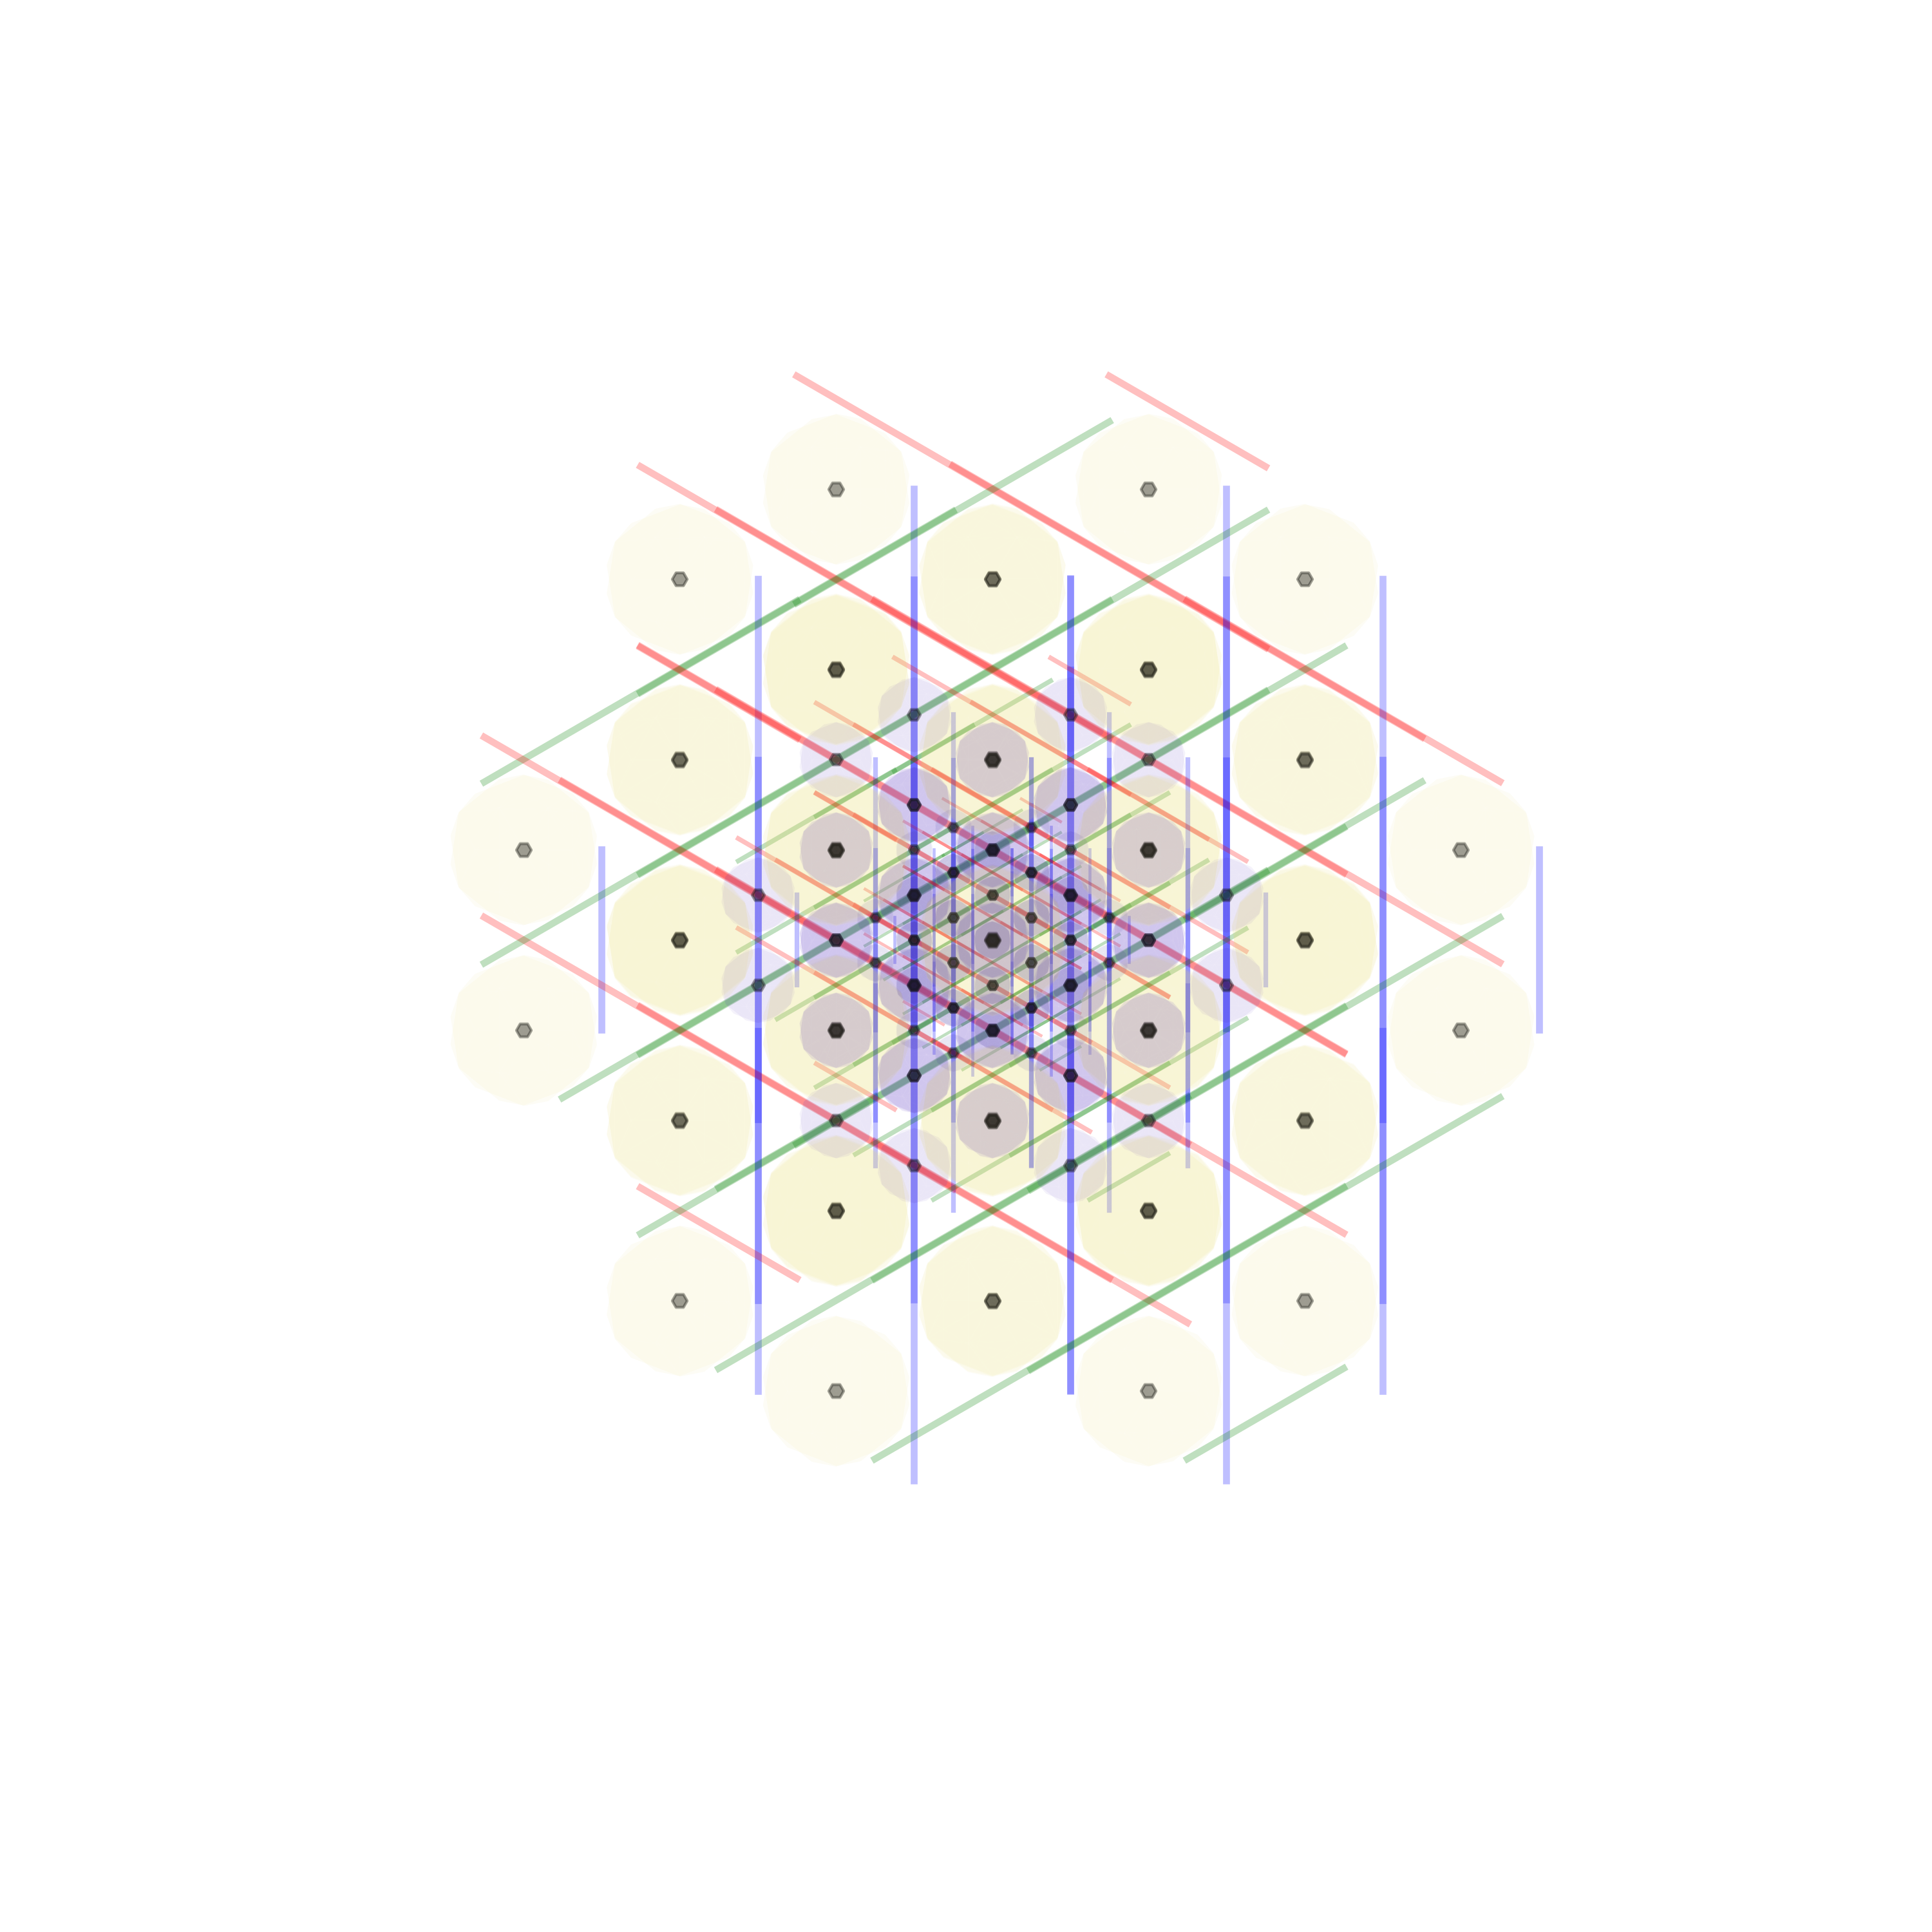
\includegraphics[trim={150 150 150 155}, scale=0.75]{fig-intro}
    \caption{Illustration of the \AAAB{} structure (\betaW{}) at three different scales, generated using \texttt{A15.py} (\texttt{fig-intro.png.txt}). The visualization highlights the constituent pyritohedral and tetradecahedral elements, demonstrating how the structure maintains its fundamental $Pm\bar{3}n$ space group symmetry while revealing increasing detail at finer resolutions.}
    \label{fig-intro}
\end{figure}

\section{Introduction: Floats, Fairness, and the A15 Foundation}\label{sec-introduction}

Binary floating-point numbers, commonly known as ``floats'' and largely governed by the IEEE 754 standard \cite{IEEE754-2019}, are the computational workhorses for representing real numbers. They offer a vast dynamic range essential for graphics and science, yet this reach often comes at the cost of precision. Floats are notorious for providing \emph{approximately correct} answers\footnote{Floats are abundant in software yet maddeningly fickle; among the first one-hundred simple reciprocals ($1/n$), ninety-three require approximation in standard binary float formats \cite{Goldberg1991}.}, representing most values inexactly. These tiny, fundamental representation errors, inherent in their structure (\Cref{eq-float-representation}), can accumulate and interact, particularly challenging the deterministic consistency required for networked virtual reality (VR) or distributed simulations. This research confronts these challenges head-on, proposing an alternative spatial representation rooted in the unique crystallographic properties of the \AAAB{} phase structure (\betaW{}, space group $Pm\bar{3}n$, No.~223 \cite{ITCVolumeA2016}), as illustrated in \Cref{fig-intro}. Furthermore, establishing a robust foundation for spatial representation with inherent numerical stability and structural consistency extends beyond immediate interactive fidelity. Such a foundation offers compelling advantages for long-term data archival, application-agnostic interoperability across diverse platforms, and the efficient decomposition and distribution of spatial computations in parallel and edge computing environments.

\subsection{The Challenge of Floating-Point Precision}\label{subsec-intro-floats}

Standard normalized binary floating-point numbers derive their value from three components: a sign bit, a biased exponent, and a significand (mantissa). Conceptually\footnote{This simplified view omits details such as exponent bias, subnormal numbers, infinities, and NaNs, rigorously defined in \cite{IEEE754-2019} but not central to the core issue of approximation.}, their value relates to:
\begin{equation} \label{eq-float-representation}
    \text{value} = (-1)^{\text{sign}} \times (1 + \text{significand}) \times 2^{\text{exponent}}
\end{equation}
The fixed-size significand offers constant \emph{relative} precision within an exponent range, while the exponent scales the value logarithmically. This design excels at exactly representing powers of two and fractions whose denominators are solely powers of two, but only a finite subset thereof. Consequently, most decimal values and even many simple fractions (e.g., $1/10$) are merely approximated \cite{Goldberg1991}.

While seemingly minuscule, these representation errors can compound, critically affecting reproducibility. In distributed systems like multiplayer games or collaborative VR, this becomes paramount. Identical logical inputs processed on different hardware architectures, operating systems, or even with different compiler optimizations can yield subtly divergent floating-point results. This variance breaks simulation consistency, undermines fairness in competition \cite{Claypool2006}, complicates debugging and verification, and fundamentally opposes the requirement for determinism. Yet, widespread hardware acceleration makes IEEE 754 formats---primarily binary32 (\SI{32}{\bit}, single-precision) and binary64 (\SI{64}{\bit}, double-precision)---ubiquitous in modern CPUs and GPUs. Binary32, in particular, remains vital for performance-sensitive applications like game development and VR, establishing a key baseline for efficiency comparisons. This work, therefore, accepts the practical necessity of floats but seeks to structure their use, mitigating risks to determinism via the disciplined partitioning and verifiable scaling offered by the \AAAB{} framework detailed in \Cref{sec-framework-design}.

\subsection{The A15 Phase Structure: A Crystallographic Foundation}\label{subsec-intro-a15}

Effectively partitioning virtual space requires a measure of geometric ``fairness''—a balance between \textbf{isometry} (preserving distances between corresponding points) and \textbf{isotropy} (uniformity of properties across different directions). Discretizing continuous space onto a lattice while preserving both ensures that spatial relationships remain consistent and free from directional bias. While regular lattices achieve perfect isometry through translational symmetry, attaining high isotropy is constrained by fundamental geometric principles. The continuous rotational symmetry group in 3D, $SO(3)$, implies that highly isotropic structures should appear locally spherical. However, the imposition of discrete translational symmetry restricts the allowed rotational symmetries to only 1-, 2-, 3-, 4-, and 6-fold axes. This is the essence of the \textbf{crystallographic restriction theorem} \cite{AshcroftMermin1976}, which explicitly forbids the global 5-fold symmetry characteristic of highly isotropic polyhedra like the icosahedron (associated with the $I_h$ point group symmetry \cite{Coxeter1973}) in periodic lattices.

The \AAAB{} structure ($Pm\bar{3}n$, No.~223 \cite{ITCVolumeA2016}) navigates this restriction with notable elegance. It is based on the simple primitive cubic ($cP$) Bravais lattice but incorporates a complex basis (or motif) containing two distinct types of crystallographic sites within its conventional unit cell \cite{FrankKasper1958, FrankKasper1959}, as illustrated in \Cref{fig-cell2}:
\begin{itemize} \itemsep0pt
    \item 25\% are C12 sites: 12-coordinated, occupying Wyckoff position 2a (e.g., at fractional coordinates $(0, 0, 0)$ and $(1/2, 1/2, 1/2)$). Their local coordination environment exhibits characteristics related to pyritohedral symmetry.
    \item 75\% are C14 sites: 14-coordinated, occupying Wyckoff position 6d (e.g., at $(1/4, 1/2, 0)$ and its symmetry equivalents \cite{ITCVolumeA2016}). Their local environment resembles a tetradecahedron (a 14-faced polyhedron).
\end{itemize}
This intricate arrangement results in a high average coordination number, calculated as $Z_{avg} = (0.25 \times 12) + (0.75 \times 14) = 13.5$, suggesting a densely connected local structure conducive to efficient packing. The local symmetry around these sites is described by the crystallographic point group $T_h$ ($m\bar{3}$, order 24). Significantly, $T_h$ is a maximal subgroup common to both the full cubic symmetry group $O_h$ (order 48) and the non-crystallographic icosahedral group $I_h$ (order 120) \cite{CoxeterMoser1972}. While lacking the forbidden 5-fold axes of $I_h$, $T_h$ retains key 3-fold rotational symmetries present in icosahedral structures. This unique symmetry allows the \AAAB{} structure to incorporate significant near-icosahedral local ordering, boosting local isotropy considerably compared to simpler cubic structures, all while maintaining the long-range periodicity required by crystallography. The structure also features alternating left- and right-handed local environments around the 6d sites, adding further complexity relevant to implementation (\Cref{subsubsec-limits-handedness}).

Crucially for this work, the canonical definition of the \AAAB{} structure relies on fractional coordinates inherently suitable for binary representation: $0$, $1/4$, and $1/2$. These values are exactly representable in base-2 systems. When these fractional coordinates are mapped onto an integer lattice (conceptually, by scaling the unit cell coordinates by 4, aligning with the derivation of the 96-unit baseline in \Cref{subsubsec-scaling-baseline}), two characteristic squared site-to-site distances emerge within this integer framework: $d^2 = 4$ (yielding distance 2) and $d^2 = 5$ (yielding distance $\sqrt{5}$). The presence of $\sqrt{5}$, the hypotenuse of a fundamental 2:1 right triangle, connects the structure's geometry directly to the golden ratio $\phi = (1+\sqrt{5})/2$, further reflecting the embedded near-icosahedral characteristics. This intrinsic numerical simplicity and compatibility with base-2 representation ensures that the \AAAB{} structure can be defined and scaled with precision, forming a robust foundation for the numerically stable encoding framework developed herein (\Cref{subsec-stability}).

\begin{figure}[!ht]
    \capstart
    \centering
    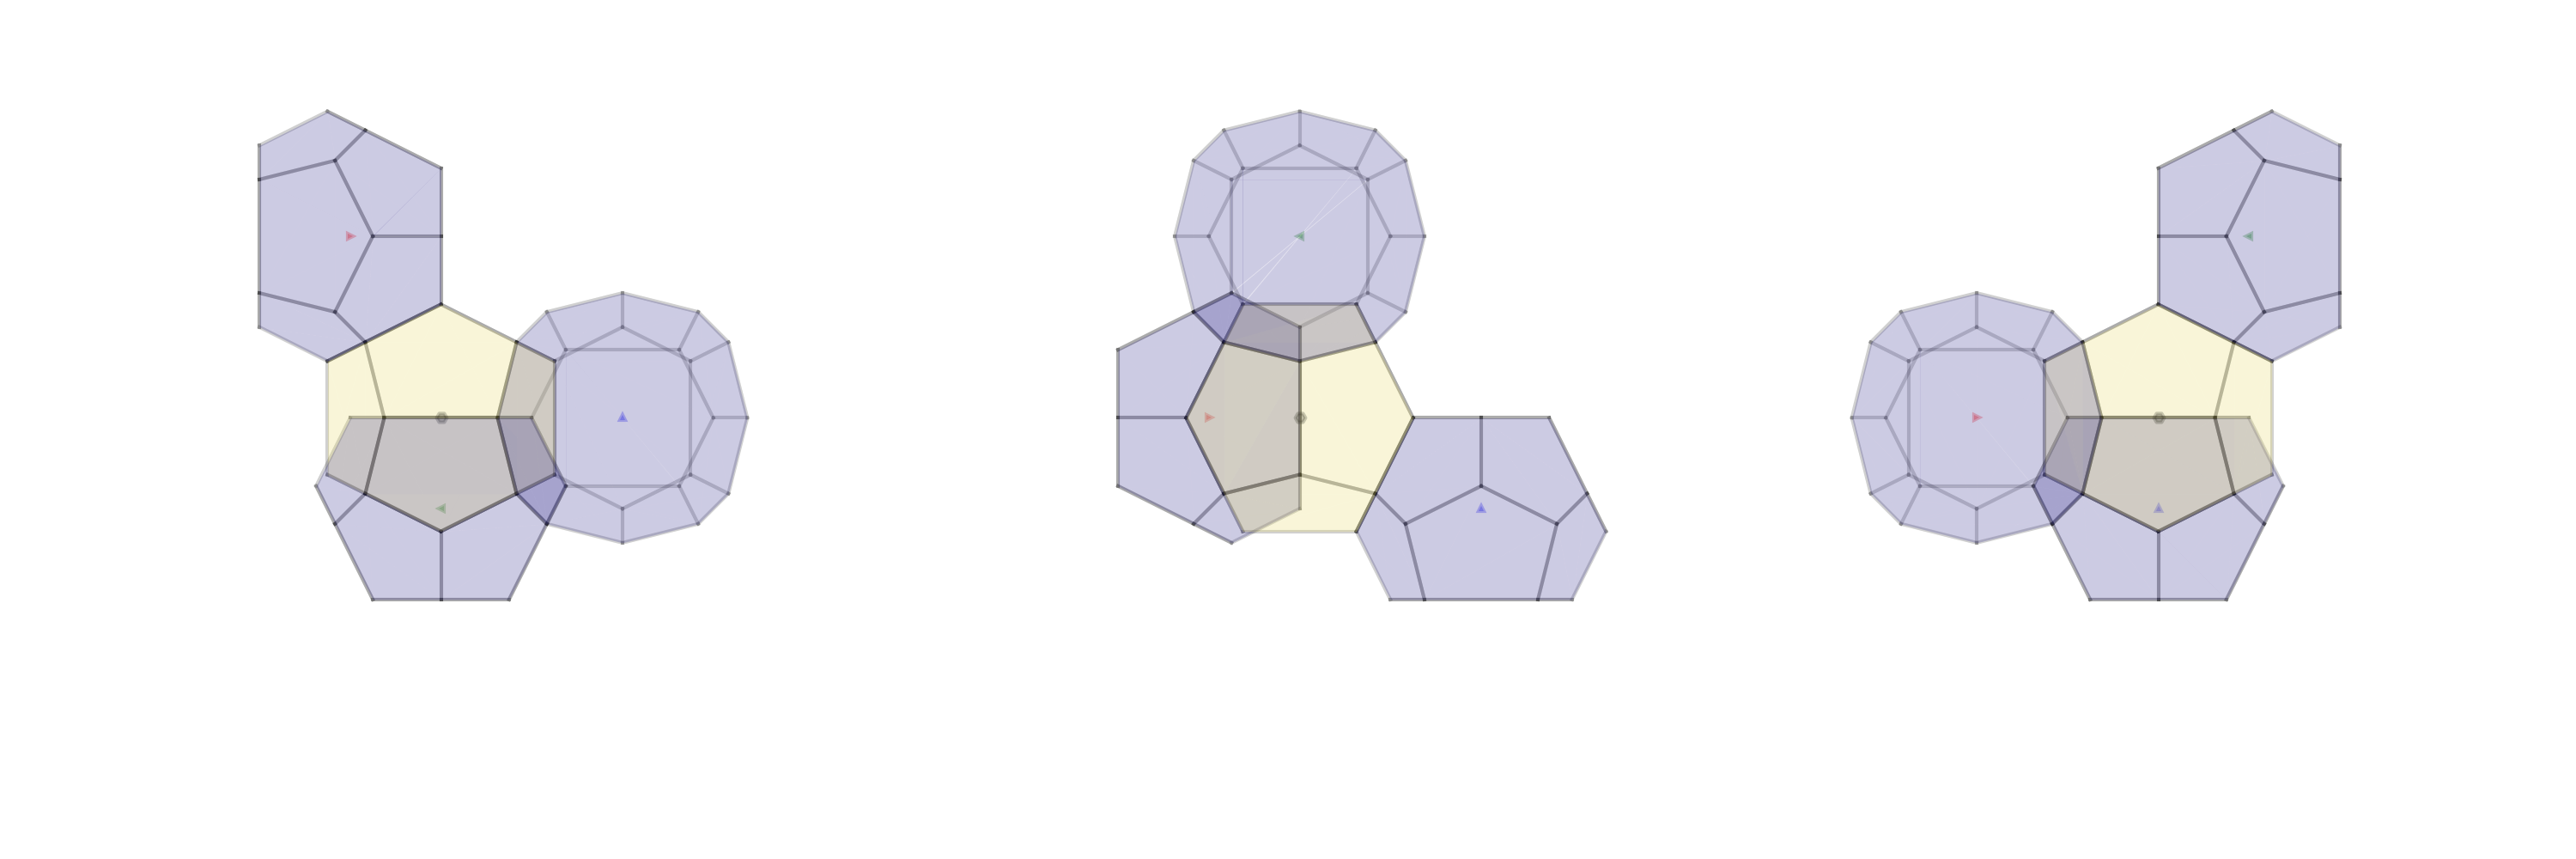
\includegraphics[trim={25 50 25 0}, scale=0.55]{fig-cell2}
    \caption{Components illustrating the local arrangement within a left-handed $^1/_2$ unit cell fragment of the \AAAB{} structure. Shows C12 (Wyckoff 2a, center of pyritohedral environment) and C14 (Wyckoff 6d, center of tetradecahedral environment) sites demonstrating the local complexity within the overall $Pm\bar{3}n$ symmetry. Generated via \texttt{A15.py} (\texttt{fig-cell2.png.txt}).}
    \label{fig-cell2}
\end{figure}

\subsection{Local Discretization Methods: WPH and TSP}\label{subsec-intro-partitioning}

While the \AAAB{} structure defines the target lattice points for coordinate encoding, mapping arbitrary continuous coordinates from a virtual environment onto these discrete identifiers requires a well-defined \emph{local discretization method}. This method effectively defines the boundaries of the region (the ``cell'') surrounding each \AAAB{} site; any continuous point falling within a given cell is quantized or mapped to that specific site's identifier. This framework primarily considers two such methods, both intrinsically linked to the \AAAB{} structure, sharing its $Pm\bar{3}n$ space group symmetry, and implemented within the accompanying \texttt{A15.py} software (\Cref{fig-wp-ts}):

\begin{description} \itemsep0.5em
    \item[\WPH{} (WPH) Geometry:] This research utilizes the geometric polyhedral form of the \WP{} structure as a partitioning method. It divides space using cells of two distinct shapes: a 12-faced pyritohedron and a 14-faced tetradecahedron, arranged in a precise 1:3 ratio \cite{WeairePhelan1994}. These cell shapes correspond topologically to the local coordination environments of the C12 and C14 sites within the \AAAB{} structure, respectively. This partitioning is notable for its high degree of isotropy, closely mirroring the symmetry characteristics of the underlying lattice. (It is important to distinguish this geometric, space-filling honeycomb from the related but distinct relaxed, minimal-surface structure which famously provided a counter-example to Kelvin's conjecture on foam partitioning \cite{Kelvin1887, Kusner1996, WeaireHutzler2001}.)
    \item[\TSP{} (TSP) Geometry:] A structurally simpler alternative partitioning method, activated within \texttt{A15.py} via the \texttt{-stix} configuration option. This method employs axis-aligned planar faces, effectively dividing space into cubic blocks centered on the \AAAB{} lattice sites. While offering computational advantages for certain operations (such as point-in-cell tests) due to its simpler geometry, this approach generally exhibits lower isotropy compared to \tWPH{} method.
\end{description}
Crucially, both \tWPH{} and \tTSP{} serve as interchangeable local discretization methods within this framework. They define the specific geometry used to quantize continuous space around each \AAAB{} lattice site. The choice influences the precise shape of these local regions and boundaries, impacting factors like the resulting partition's isotropy and the computational cost of the quantization step itself. However, the fundamental coordinate identifier that is ultimately transmitted or stored remains based on the position within the underlying \AAAB{} lattice, regardless of which local method is used for the mapping.

\begin{figure}[!ht]
    \capstart
    \centering
    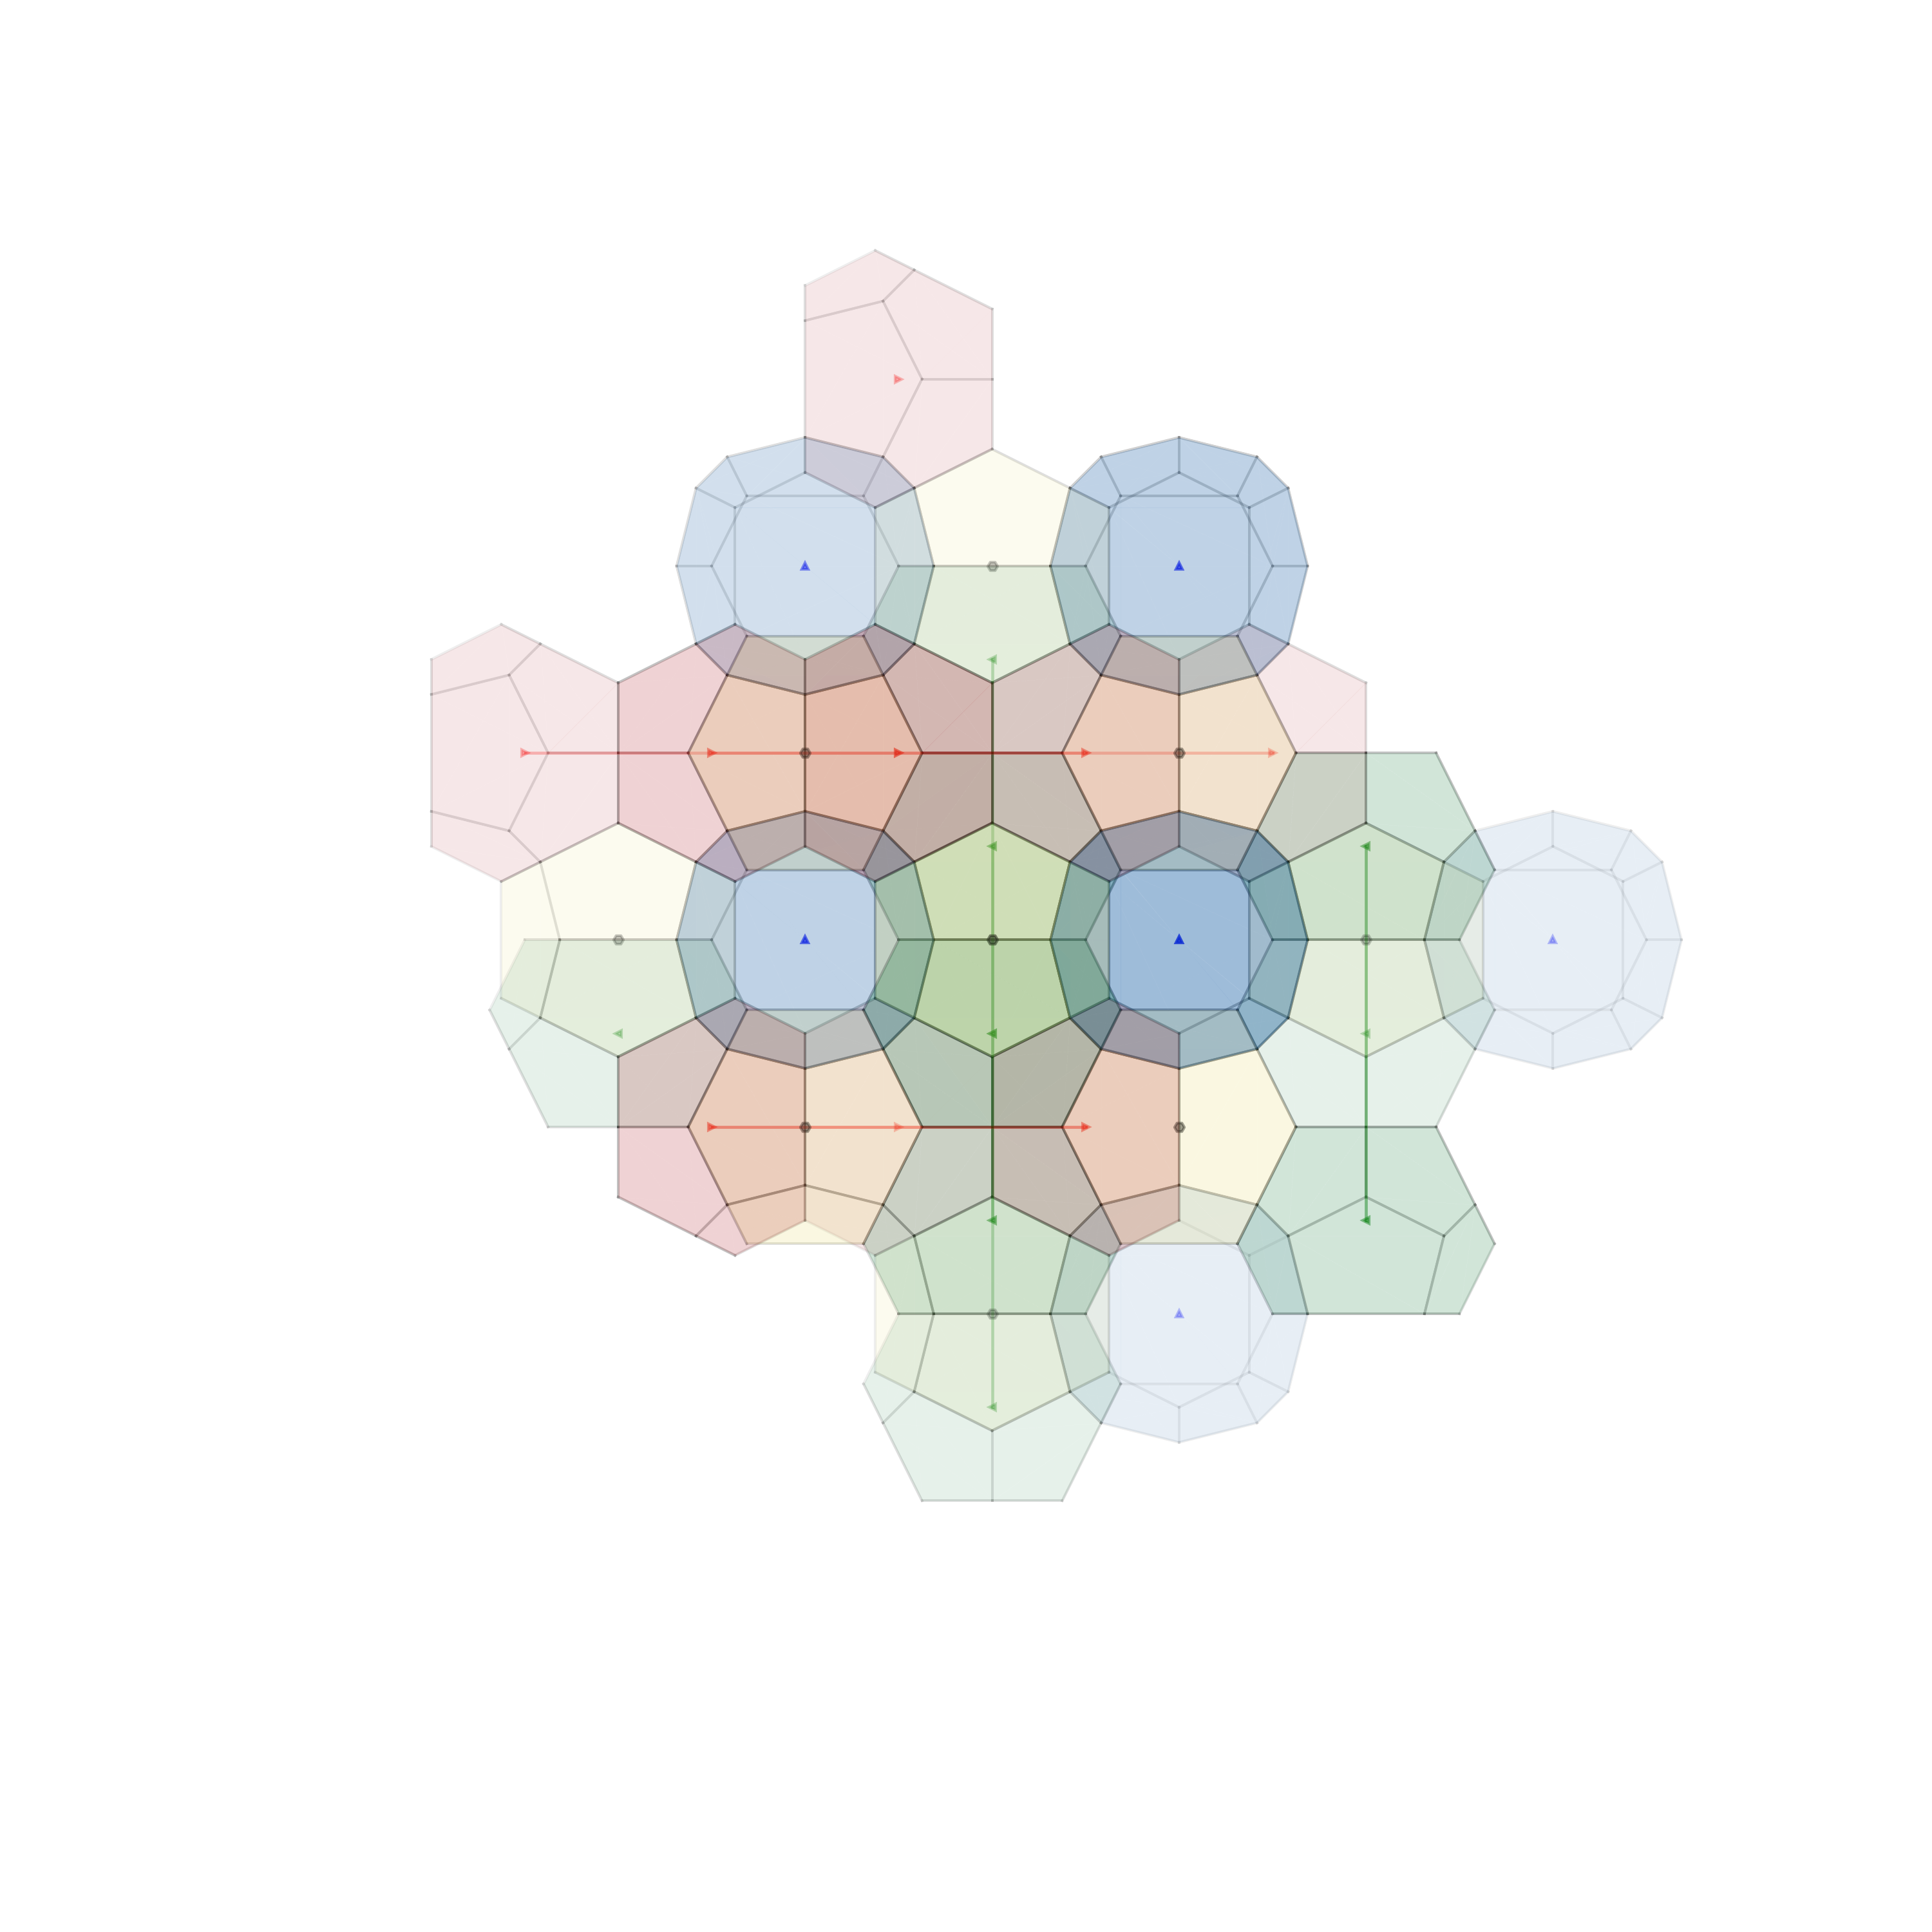
\includegraphics[trim={130 140 80 50}, scale=0.35]{fig-wp}%
    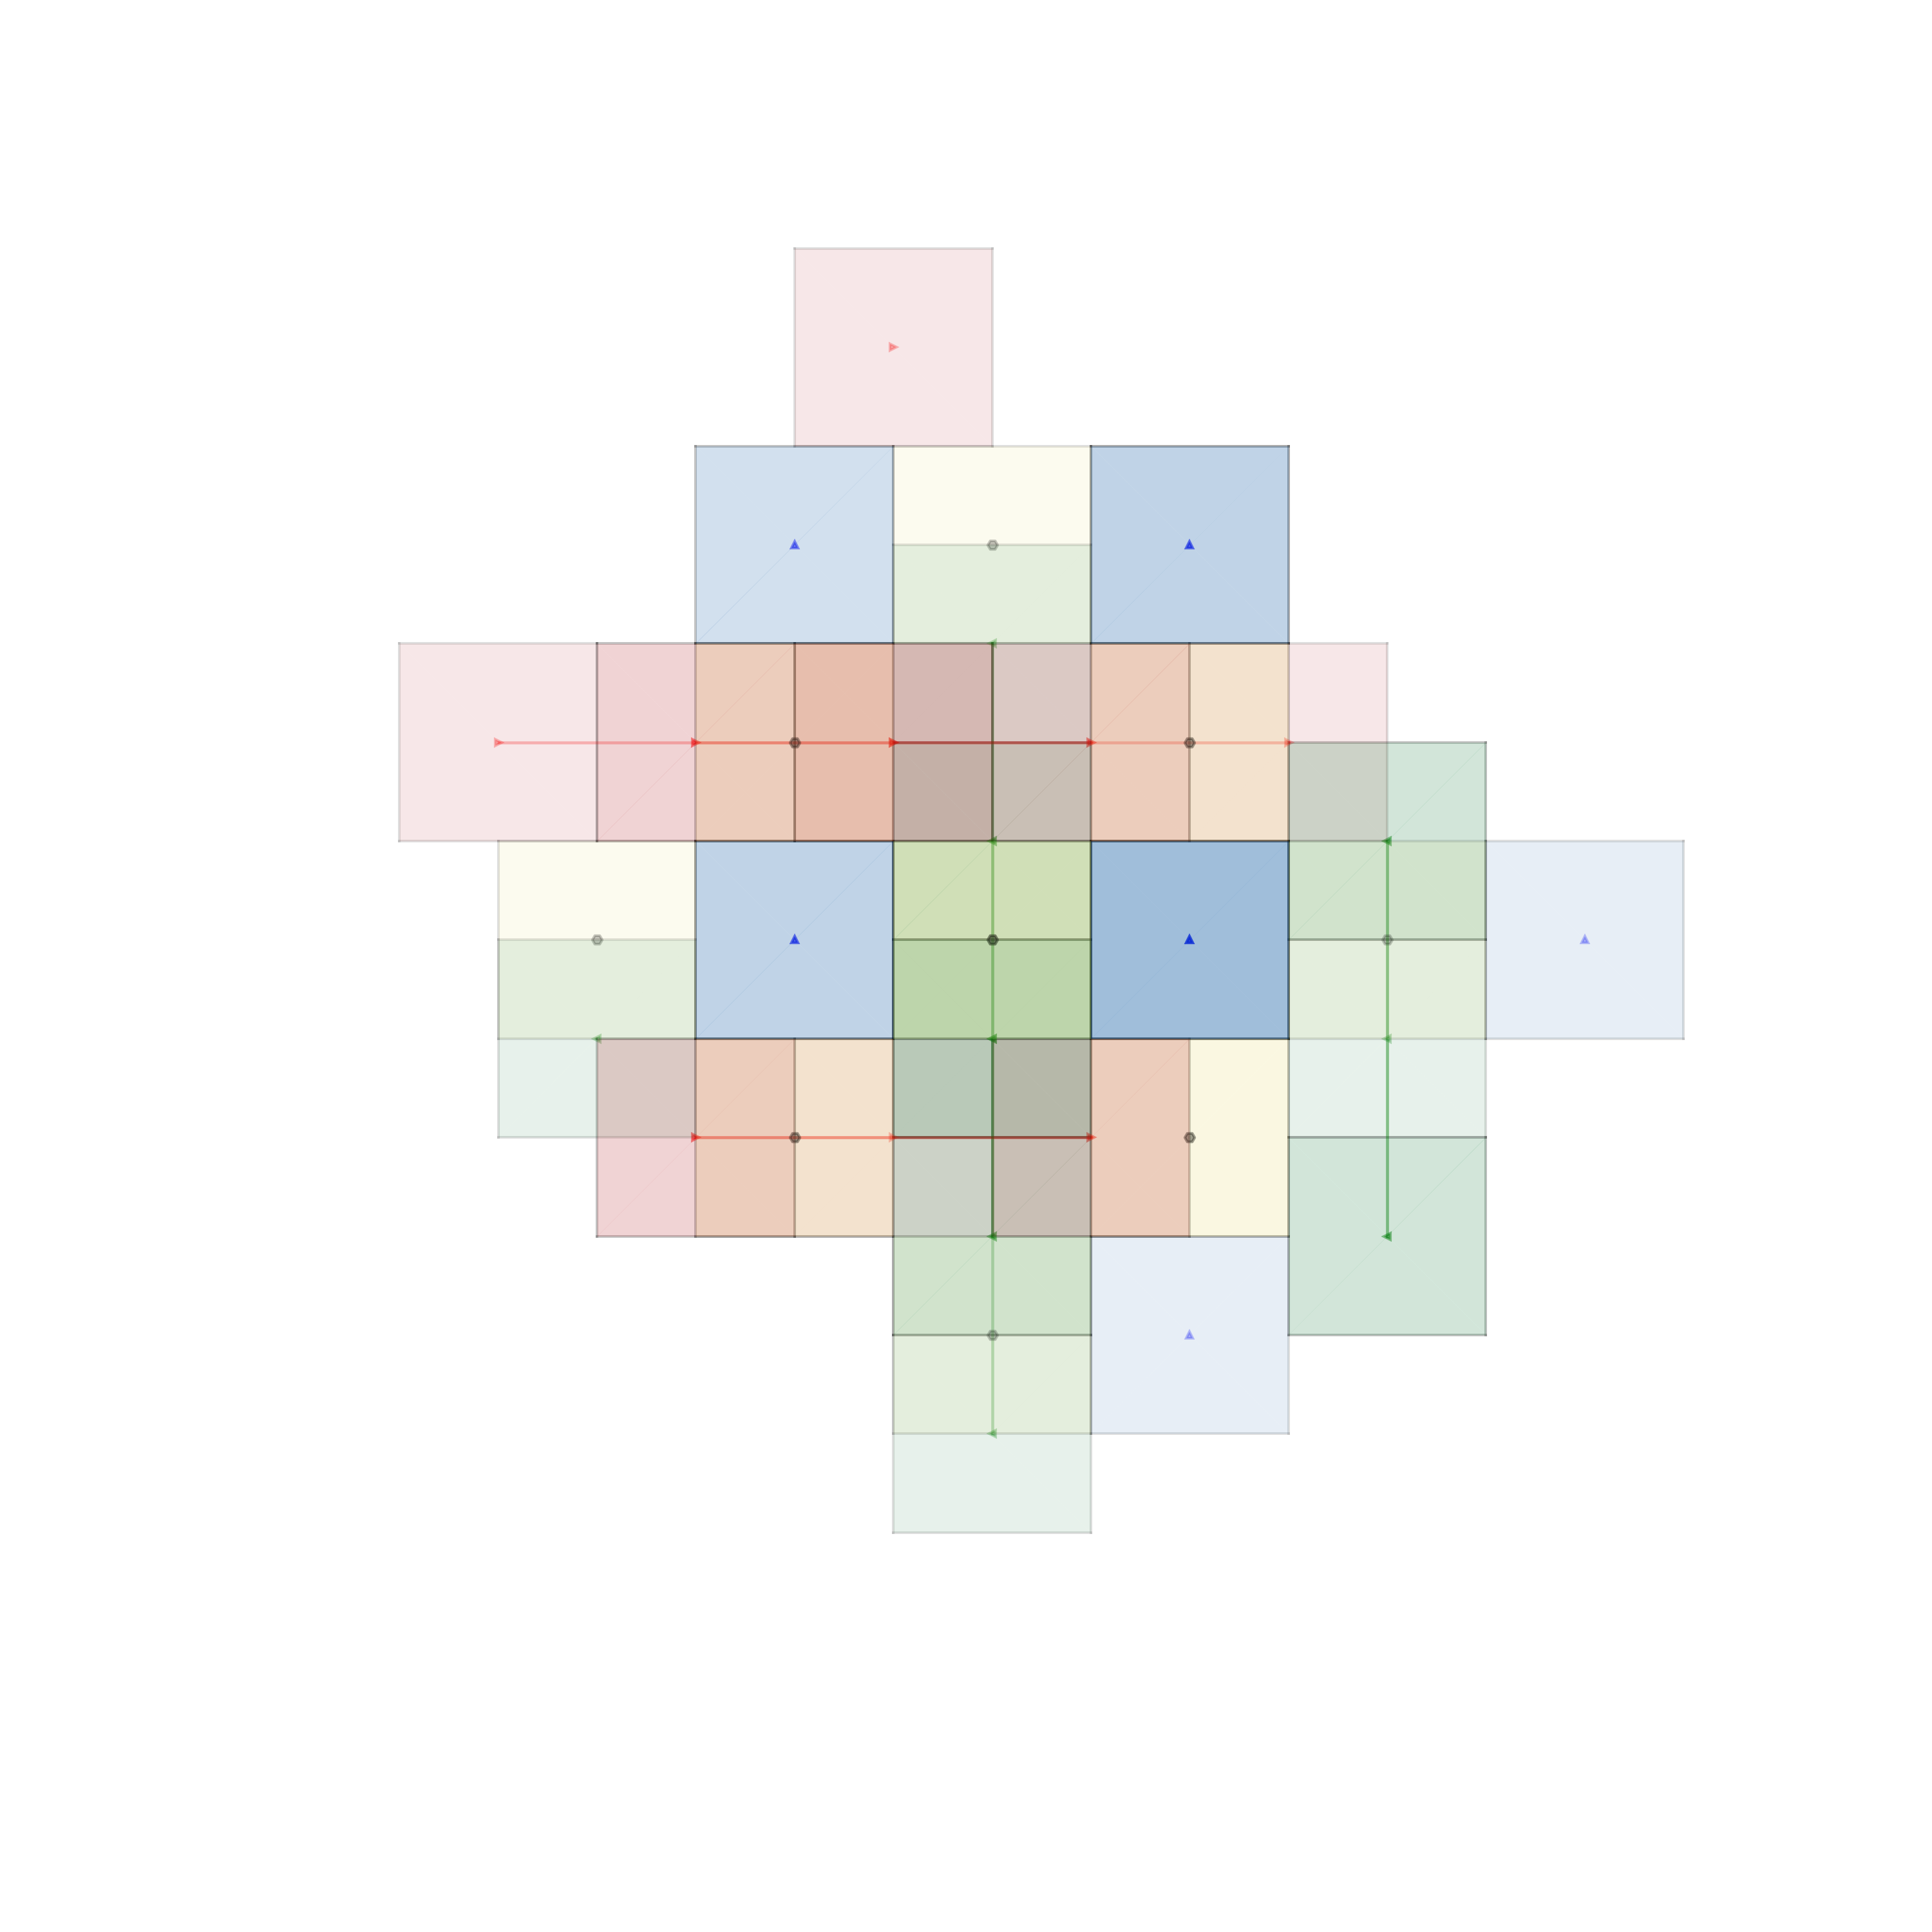
\includegraphics[trim={130 140 80 50}, scale=0.35]{fig-ts}
    \caption{Visualization of local discretization methods related to the underlying \AAAB{} structure. Left: The geometric polyhedral variant of the \textbf{\WPH{}}, featuring pyritohedra (12 faces) and tetradecahedra (14 faces). Right: The simpler \textbf{\TSP{}} partitioning using axis-aligned planar faces resulting in cubic blocks centered on \AAAB{} sites. Both share the $Pm\bar{3}n$ space group symmetry. Generated using \texttt{A15.py} (\texttt{fig-wp.png.txt} and \texttt{fig-ts.png.txt}).}
    \label{fig-wp-ts}
\end{figure}

\subsection{Distinction from Traditional Spatial Indexing}\label{subsec-comparison-indexing}

The \AAAB{}-based partitioning approach presented here relates to, yet fundamentally differs from, traditional spatial indexing techniques commonly employed in databases, geographic information systems (GIS), and various domains of computer graphics (e.g., octrees \cite{Finkel1974}, R-trees \cite{Guttman1984}, k-d trees \cite{Bentley1975}; see \cite{Samet1990} for a comprehensive overview). Conventional indexing methods typically utilize data-driven, adaptive strategies; their partitioning boundaries often adjust dynamically based on the distribution and density of existing spatial objects, with the primary goal of optimizing query performance (such as range searches or nearest neighbor lookups) for that specific dataset.

In stark contrast, the \AAAB{} framework imposes a predetermined, regular, crystallographically-inspired structure onto the virtual space itself, largely independent of the dynamic content residing within it. This \emph{structure-first} methodology prioritizes the creation of a universal, efficient, and geometrically sound fabric for spatial representation and encoding. The key distinctions are summarized in \Cref{tab-comparison-indexing}. The \AAAB{} approach deliberately trades the dynamic query optimization focus of traditional indexing for significant advantages in predictability, communication efficiency (via compact identifiers that implicitly encode the regular structure), guaranteed numerical determinism (when using stable scaling regimes), and inherent geometric consistency derived from crystallographic symmetry—properties particularly valuable for networked virtual environments demanding shared spatial understanding, robustness against floating-point discrepancies, and efficient state synchronization.

\begin{table}[!ht]
\centering
\caption{Comparison of Spatial Organization Approaches.}
\label{tab-comparison-indexing}
\begin{tabularx}{\textwidth}{>{\raggedright\arraybackslash}p{0.21\textwidth} >{\raggedright\arraybackslash}p{0.38\textwidth} >{\raggedright\arraybackslash}X}
\toprule
\textbf{Characteristic} & \textbf{Traditional Spatial Indexing}\newline (e.g., Octree \cite{Finkel1974}, R-tree \cite{Guttman1984}, k-d tree \cite{Bentley1975}) & \textbf{\AAAB{} Crystallographic Partitioning} \\
\midrule
Main Objective & Efficient query/retrieval of existing, often arbitrary, data & Uniform, deterministic spatial discretization and efficient coordinate encoding \\ \addlinespace
Partition Strategy & Data-driven; adaptive boundaries; often hierarchical; structure follows data & Structure-driven; regular lattice; predetermined boundaries (via WPH/TSP local methods); data follows structure \\ \addlinespace
Symmetry Awareness & Generally low; structure adapts to data, often breaking ambient symmetries & High; leverages crystallographic symmetry ($T_h$, $Pm\bar{3}n$) of the imposed lattice \\ \addlinespace
Coordinate Handling & Typically preserves input precision (e.g., float coordinates) & Quantizes coordinates to discrete representations (\AAAB{} identifiers, often integers) \\ \addlinespace
Memory Usage & Variable, depends on data density/distribution; includes tree/node overhead & Predictable based on defined scale/volume; highly efficient storage using integer identifiers \\ \addlinespace
Isotropy & Variable; depends heavily on data distribution and algorithm specifics & High local isotropy inherent in the \AAAB{} structure, especially when using \WPH{} partitioning \\ \addlinespace
Neighborhood Info & Requires explicit tree traversal or complex range/proximity queries & Implicit, regular neighbor relationships directly derivable from the lattice structure \\ \addlinespace
Temporal Stability & Partitioning structure can change significantly as data moves or updates & Fixed partitioning grid provides temporal coherence for coordinate mapping (though content moves within) \\ \addlinespace
Determinism Guarantee & Generally low; susceptible to float variance affecting boundary tests/traversal & High; guaranteed bit-level consistency achievable with stable scaling regimes ($\epsilon_\Delta = 0$) \\ \addlinespace
Main Use Case & Databases, GIS \cite{Samet1990}, dynamic collision detection, view frustum culling & Foundational spatial fabric for deterministic VR/simulations, compact coordinate encoding, networked state consistency, verifiable replays \\
\bottomrule
\end{tabularx}
\end{table}

\subsection{Comparative Context: Other Symmetric Structures}\label{subsec-comparison-structures}

The 230 crystallographic space groups categorize all possible ways to combine periodic translational symmetry (defined by the 14 Bravais lattices) with rotational and reflectional symmetries (defined by the 32 crystallographic point groups) in 3D space \cite{ITCVolumeA2016}. Situating the \AAAB{} structure (space group $Pm\bar{3}n$, No.~223) within this framework highlights its distinctive characteristics relevant to packing and partitioning (\Cref{tab-spacegroups}).

\begin{table}[!ht]
    \centering
    \caption{Comparison of Relevant Cubic Space Groups.}
    \label{tab-spacegroups}
    \begin{tabular}{l c c c c l}
        \toprule
        \textbf{Structure Type} & \textbf{No.} & \textbf{HM Symbol} & \textbf{Point Group} & \textbf{Order} & \textbf{Bravais Lattice} \\
        \midrule
        \textbf{\AAAB{} Type}  & \textbf{223} & $\boldsymbol{Pm\bar{3}n}$ & $\boldsymbol{m\bar{3}}$ $\boldsymbol{(T_h)}$ & \textbf{24} & \textbf{Primitive (cP)} \\ \addlinespace
        Simple Cubic (SC)      & 221          & $Pm\bar{3}m$              & $m\bar{3}m$ $(O_h)$                  & 48             & Primitive (cP) \\
        BCC Type (e.g., W)     & 229          & $Im\bar{3}m$              & $m\bar{3}m$ $(O_h)$                  & 48             & Body-Centered (cI) \\
        FCC Type (e.g., Cu)    & 225          & $Fm\bar{3}m$              & $m\bar{3}m$ $(O_h)$                  & 48             & Face-Centered (cF) \\
        \bottomrule
    \end{tabular}
    \vspace*{0.5ex}
    \par
    \footnotesize Data sourced from International Tables for Crystallography, Vol A \cite{ITCVolumeA2016}. HM Symbol: Hermann-Mauguin notation.
\end{table}

As shown, \AAAB{}'s $Pm\bar{3}n$ space group utilizes the primitive cubic ($cP$) Bravais lattice but applies the $T_h$ point group symmetry (order 24). This group possesses lower overall symmetry than the full cubic $O_h$ group (order 48) characteristic of the highest-symmetry simple cubic, body-centered cubic (BCC, $cI$), and face-centered cubic (FCC, $cF$) structures. However, as discussed (\Cref{subsec-intro-a15}), the specific $T_h$ symmetry is significant because it represents a maximal crystallographic subgroup linking cubic ($O_h$) and non-crystallographic icosahedral ($I_h$) symmetries \cite{CoxeterMoser1972}. This unique combination allows the \AAAB{} structure to accommodate its complex basis with distinct C12 and C14 sites, enabling its exceptionally high average coordination number (13.5), which relates to efficient local packing and high connectivity.

When compared to common space-filling honeycombs and related sphere packings, the \AAAB{} structure, particularly when coupled with \tWPH{} partitioning method, offers further distinctions relevant to this framework:
\begin{description} \itemsep0.5em
    \item[vs. BCC-derived Structures:] The body-centered cubic lattice (BCC, coordination number Z=8) and its dual, the bitruncated cubic honeycomb (Kelvin's structure \cite{Kelvin1887}), have lower fundamental coordination than \AAAB{} (13.5), suggesting a less densely connected local environment.
    \item[vs. FCC-derived Structures:] The face-centered cubic lattice (FCC, coordination Z=12) represents the densest packing of identical spheres \cite{ConwaySloane1999} and is related to the rhombic dodecahedral honeycomb. While achieving maximal coordination for identical points, \AAAB{} surpasses this average by utilizing two distinct, efficiently arranged site types.
    \item[vs. \tWPH{}:] The geometric \WPH{}, used as a local discretization method, shares the $Pm\bar{3}n$ space group and its cell types correspond topologically to the A15 site environments. This ensures the partitioning boundaries naturally align with the symmetries and neighborhood relationships of the underlying A15 encoding lattice, a unique synergy not offered by partitions derived from simpler lattices.
\end{description}
In summary, the unique combination offered by the \AAAB{} structure—its high mean coordination, significant local isotropy via $T_h$ symmetry, a direct relationship to the compatible \WPH{} partitioning structure, and inherently binary-suitable base coordinates—makes it exceptionally well-suited for the deterministic, efficient, and geometrically sound spatial encoding framework proposed here.

\section{The \AAAB{} Encoding Framework: Design and Implementation}\label{sec-framework-design}

The heart of this research lies in translating the idealized crystallographic description of the \AAAB{} structure (\Cref{subsec-intro-a15}) into a practical, numerically robust system for partitioning continuous 3D space and encoding coordinates. This requires establishing an appropriate and consistent scale, mapping continuous coordinates to discrete lattice identifiers, and ensuring the process avoids the pitfalls of floating-point approximation (\Cref{subsec-intro-floats}). The framework achieves this through a carefully staged approach to coordinate scaling, primarily operating within an internal integer coordinate system during geometric construction to preserve fidelity and defer floating-point conversion until the final output step. This section details this methodology and introduces the reference implementation, \texttt{A15.py} \cite{Risinger2024A15}, used throughout this work for generation, analysis, and validation.

\subsection{Core Principle: Internal Integer Representation}\label{subsec-scaling-framework}

Applying a discrete lattice like \AAAB{} to represent continuous space necessitates a rigorous scaling framework. Simply using floating-point coordinates throughout the geometric construction risks introducing the very numerical inconsistencies the framework aims to eliminate. Therefore, the methodology prioritizes calculations within a well-defined internal integer coordinate system, delaying the mapping to inexact output formats until the final step. This preserves the precise geometric relationships inherent in the \AAAB{} structure and forms the bedrock for numerical stability. Crucially, this reliance on an internal integer foundation, particularly when an application deliberately aligns its native coordinate system and units with a chosen stable A15 scale ($\epsilon_\Delta = 0$, \Cref{subsubsec-stability-diff}), opens pathways for highly efficient quantization. In such aligned scenarios, mapping continuous or application-native coordinates to A15 identifiers may simplify significantly, potentially reducing complex geometric searches to fast integer arithmetic operations like truncation or bit shifts, thereby mitigating concerns about quantization overhead through careful co-design.

\subsection{Multi-Stage Scaling Pipeline}\label{subsec-scaling-pipeline}

The conversion from the abstract \AAAB{} definition to concrete coordinates involves a systematic, multi-stage pipeline implemented within \texttt{A15.py}. This process uses several interacting parameters and fixed factors to progressively build the structure within the internal integer system before final output scaling. The key stages are detailed below, and the parameters are summarized in \Cref{tab-scaling-params}.

\subsubsection{Primitive Definition and Resolution (\texttt{prescale})}\label{subsubsec-scaling-prescale}
The pipeline originates with the definition of the fundamental geometric units associated with the \AAAB{} basis sites—typically the pyritohedra and tetradecahedra related to the \WPH{} method (\Cref{subsec-intro-partitioning}), or the cubic blocks for the \TSP{} method. Functions within \texttt{A15.py} (e.g., \texttt{pyritohedron()}, \texttt{tetradecahedra()}) apply an internal integer multiplier, the \texttt{prescale} parameter, to the canonical \emph{dimensionless fractional} coordinates (like $0, 1/4, 1/2$) defining the vertices of these shapes. This crucial first step converts the fractional values into \emph{primitive-relative integer coordinates}, establishing the minimum resolution necessary to accurately represent the individual geometric primitives without internal approximation. Default \texttt{prescale} values in \texttt{A15.py} (typically \num{20} for standard WPH-derived shapes, \num{24} for TSP-derived shapes via \texttt{-stix}) are chosen specifically to ensure these base vertices land precisely on an integer grid relative to the shape's center.

\subsubsection{Lattice Placement (Factor 24)}\label{subsubsec-scaling-lattice}
The \texttt{lattice()} function in \texttt{A15.py} replicates these integer-vertex polyhedra periodically across 3D space according to the $Pm\bar{3}n$ symmetry rules. It determines the positions for the \emph{centers} of these polyhedra based on \emph{integer lattice vectors} \texttt{xyz} relative to an origin offset \texttt{o}. A key element in this placement is the fixed \textbf{Lattice Spacing Factor of 24 units}. Within the \texttt{lattice()} function, the calculation \texttt{(xyz + o) * 24} multiplies the integer lattice vector by this factor. This defines the spacing between the nominal lattice points (i.e., the centers of the polyhedra) \emph{measured in the integer units established by \texttt{prescale}}. This factor ensures the correct relative positioning of the repeating units within the overall \AAAB{} lattice framework.

\subsubsection{Basis Accommodation (Factor 96 Baseline)}\label{subsubsec-scaling-baseline}
The \AAAB{} structure's complexity arises from its multi-atom basis; it contains distinct crystallographic sites (Wyckoff 2a and 6d) not just at the nominal lattice points defined above, but also at specific fractional offsets, notably involving $1/4$ for the 6d sites. To place \emph{all} required sites onto a single, consistent internal integer grid requires a resolution finer than the 24-unit spacing factor alone provides. The smallest denominator involved is 4 (from $1/4$). Therefore, the internal integer grid must be conceptually scaled such that one unit step along a primitive lattice vector corresponds to $4 \times 24 = 96$ internal integer units along each principal axis.

This derived \textbf{Effective Lattice Unit Factor of 96} represents the fundamental period or effective unit dimension of the comprehensive internal integer grid required to represent the \emph{complete} \AAAB{} structure (including its basis) without loss of precision due to these fractional offsets. This factor of 96 establishes the crucial \textbf{baseline dimension} relative to which the structure's inherent numerical precision requirements ($\epsilon_N$, see \Cref{subsubsec-stability-epsilon-n}) are determined and against which the final output scale ($\epsilon_\delta$) is compared for stability analysis.

\subsubsection{Optional Binary Rescaling (\texttt{rescale})}\label{subsubsec-scaling-rescale}
Before the lattice generation stage fully populates the internal integer coordinates, an optional power-of-two scaling factor, \texttt{rescale}, can be applied. This factor is specified via the \texttt{-rescale} command-line flag or implicitly through `+/-` suffixes appended to shape names in the input (e.g., \texttt{pyritohedra++} implies a rescale factor of $2^2=4$ in \texttt{A15.py}). This \texttt{rescale} factor multiplies the effective size represented by the internal integer coordinates relative to the 96-unit baseline established above. It allows adjustments to the overall size or relative proportions of different generated components \emph{before} the final output scaling step, operating purely in powers of two within the integer domain. Importantly, the choice of \texttt{rescale} influences the resulting inherent base scale $\epsilon_N$ of the internal geometry.

\subsubsection{Resultant Internal Integer Coordinates}\label{subsubsec-scaling-internal}
The cumulative effect of the initial \texttt{prescale} (\Cref{subsubsec-scaling-prescale}), the lattice placement logic (\Cref{subsubsec-scaling-lattice}, establishing the 96-unit effective baseline \Cref{subsubsec-scaling-baseline}), and any applied \texttt{rescale} factor (\Cref{subsubsec-scaling-rescale}) collectively defines the complete set of vertex coordinates for the entire generated structure. These coordinates exist within a consistent, potentially large-valued, \emph{internal integer} system referenced against the 96-unit effective lattice baseline. By prioritizing integer arithmetic throughout these construction stages, \texttt{A15.py} preserves the precise geometric relationships inherent in the \AAAB{} structure, deferring any floating-point approximation until the very last output step. This internal integer representation forms the bedrock for the numerical stability analysis detailed next.

Furthermore, the explicit control over scale inherent in this pipeline naturally supports hierarchical or multi-scale representations via relative addressing. This allows, for instance, coarse-grained coordinates identifying an entity's global position to coexist efficiently with fine-grained coordinates defining its internal details (e.g., limb articulations relative to a centroid), each utilizing an appropriate A15 scale ($\epsilon_\delta$) within the same unified structural logic, optimizing both data density and precision.

\begin{table}[!ht]
\centering
\caption{Summary of Key Scaling Parameters and Factors in \texttt{A15.py}.}
\label{tab-scaling-params}
\begin{tabularx}{\textwidth}{>{\raggedright\arraybackslash}p{0.18\textwidth} >{\raggedright\arraybackslash}X}
\toprule
\textbf{Parameter/Factor} & \textbf{Role and Implementation in \texttt{A15.py}} \\
\midrule
\texttt{prescale} & Internal integer multiplier applied within shape functions (e.g., \texttt{pyritohedron()}). Converts base fractional coordinates (0, 1/4, 1/2, etc.) to integer vertices relative to shape center. Establishes primitive resolution (Defaults: \num{20} WPH, \num{24} TSP). \\ \addlinespace
Lattice Spacing Factor (\num{24}) & Fixed factor used in \texttt{lattice()}. Multiplies integer lattice vectors \texttt{xyz} to determine nominal lattice point positions relative to origin offset \texttt{o}, measured in units defined by \texttt{prescale}. \\ \addlinespace
Effective Lattice Unit Factor (\num{96}) & Derived factor ($4 \times 24 = 96$). Represents the fundamental period of the internal integer grid along a principal axis needed to accommodate \AAAB{} basis site offsets (like 1/4) precisely. \textbf{This is the internal baseline dimension} relative to which inherent precision $\epsilon_N$ and output scale $\epsilon_\delta$ are compared. \\ \addlinespace
\texttt{rescale} & Optional pre-generator power-of-two scaling (via \texttt{-rescale} flag or \texttt{+/-} suffixes). Multiplies internal integer coordinates, adjusting size relative to the 96-unit baseline \textit{before} final output scaling. Affects the resulting $\epsilon_N$. \\ \addlinespace
\texttt{scale} ($\epsilon_\delta$) & Final global scaling factor (\texttt{-scale=<value>}) applied by \texttt{figure()} after internal integers are generated. Maps internal integers (relative to the 96-unit baseline) to output coordinates (typically float). Sets real-world size and determines numerical stability regime ($\epsilon_\Delta$) by comparison with $\epsilon_N$. Accepts various formats (integer, fraction, power, float). \\ \addlinespace
\texttt{n} & Controls lattice extent (\texttt{-n=<value>}). Integer specifies cuboid dimensions (number of lattice cells defined by the 96-unit baseline along axes); float specifies a spherical radius cutoff based on lattice vector magnitude relative to the origin. \\
\bottomrule
\end{tabularx}
\end{table}

\subsection{Numerical Stability: Regimes and Validation}\label{subsec-stability}

Achieving deterministic spatial representation—ensuring that identical logical operations yield bit-identical results across different systems—is a primary motivation for this framework. This guarantee hinges critically on the relationship between the scale chosen for the final output coordinates ($\epsilon_\delta$) and the inherent precision requirements ($\epsilon_N$) of the underlying \AAAB{} geometry, as captured by the internal integer representation (\Cref{subsec-scaling-framework}). The framework defines specific, verifiable conditions under which the mapping from the precise internal structure to the output coordinate system can be performed without introducing floating-point approximation errors relative to that internal structure.

\subsubsection{Global Output Scaling Factor ($\epsilon_\delta$)}\label{subsubsec-stability-epsilon-d}
The primary user control over the final representation's physical scale or resolution is the \texttt{scale} parameter, specified via the \texttt{-scale=<value>} command-line option in \texttt{A15.py}. We denote this crucial factor as $\epsilon_\delta$. It is applied globally by the \texttt{figure()} function \emph{after} all internal integer coordinates (relative to the 96-unit baseline) have been generated. This $\epsilon_\delta$ defines the mapping from the dimensionless internal integer system to the output coordinate system (typically floating-point). Therefore, $\epsilon_\delta$ effectively sets the real-world size represented by one unit of the internal 96-unit baseline dimension, and its specific value is the key determinant of the resulting numerical stability regime.

\subsubsection{Inherent Base Scale ($\epsilon_N$)}\label{subsubsec-stability-epsilon-n}
The internal integer geometry produced by the construction process (\Cref{subsec-scaling-pipeline}) possesses an intrinsic precision limit relative to the 96-unit baseline. This limit arises from the specific combination of the \AAAB{} basis site coordinates (involving factors of $1/4$), the chosen \texttt{prescale} value, and any applied \texttt{rescale} factor. We define $\epsilon_N$ as the \textbf{inherent base scale} required to represent this specific internal geometry exactly when mapped to a base-2 representation. Conceptually, $\epsilon_N$ is the finest scaling factor, expressible as a power of two ($1/2^N$ for some integer $N$), that allows all generated internal integer vertex coordinates to be represented perfectly as rational numbers without approximation when measured against the 96-unit baseline. It captures the structure's intrinsic geometric precision limit within the binary system used by floating-point numbers. The \texttt{A15.py} script computationally infers $\epsilon_N$ by analyzing the power-of-two denominators required for the exact rational representation of the generated internal integer geometry relative to the 96-unit baseline.

\subsubsection{Stability Condition and Difference ($\epsilon_\Delta$)}\label{subsubsec-stability-diff}
Numerical stability is achieved if, and only if, the chosen global output scale ($\epsilon_\delta$) is commensurate with the inherent base scale ($\epsilon_N$). Specifically, the mapping from the internal integer representation to the output coordinate system is guaranteed to be exact (free from representation error relative to the internal grid) if $\epsilon_\delta$ is a positive integer multiple ($m$) of $\epsilon_N$. The \texttt{A15.py} script quantifies this relationship by calculating the \textbf{stability difference}, $\epsilon_\Delta$. Conceptually, $\epsilon_\Delta$ measures the mismatch or residual error when checking if $\epsilon_\delta$ aligns perfectly with the grid defined by $\epsilon_N$:
\begin{equation}\label{eq-stability-condition}
\text{Stability Condition:} \quad \epsilon_\Delta = 0 \quad \iff \quad \epsilon_\delta = m \cdot \epsilon_N \quad \text{for some integer } m \ge 1
\end{equation}
If this condition holds ($\epsilon_\Delta = 0$), the framework operates in a stable regime. Otherwise ($\epsilon_\Delta \neq 0$), the scaling is unstable, and approximation errors are necessarily introduced relative to the internal structure.

\subsubsection{Stability Regimes}\label{subsubsec-stability-regimes}
The stability condition leads to three distinct operational regimes:

\begin{description} \itemsep0.5em
    \item[Binary Scaling ($\epsilon_\Delta = 0$ with $m=1$):] This optimal regime occurs when the chosen output scale precisely matches the minimum required inherent base scale ($\epsilon_\delta = \epsilon_N$). All internal integer coordinates map directly and exactly onto the binary floating-point grid defined by $\epsilon_N = 1/2^N$ without any approximation relative to the internal structure.
    \begin{equation}\label{eq-scaling-binary}
    \textbf{Binary}: \quad \epsilon_\delta = \epsilon_N = \frac{1}{2^N} \quad \implies \quad \epsilon_\Delta = 0
    \end{equation}
    This represents the most compact scale that allows exact representation and guarantees determinism. The validation histogram (\Cref{fig-hist}, left) shows a single, sharp peak at the exponent $-N$.

    \item[Stable Scaling ($\epsilon_\Delta = 0$ with $m > 1$):] This regime occurs when the output scale is an exact positive integer multiple ($m$) of the inherent base scale ($\epsilon_\delta = m \cdot \epsilon_N$). All internal coordinates still map exactly to representable binary floating-point values without approximation error relative to this scaled grid.
    \begin{equation}\label{eq-scaling-stable}
    \textbf{Stable}: \quad \epsilon_\delta = m \cdot \epsilon_N = \frac{m}{2^N}, \quad m \in \mathbb{Z}^+, m > 1 \quad \implies \quad \epsilon_\Delta = 0
    \end{equation}
    This regime maintains perfect representability and determinism while providing flexibility in choosing the overall physical scale. The smallest resolvable difference (Unit of Least Precision, \Cref{subsubsec-notes-ulp}) corresponds to $m$ units at the $\epsilon_N$ scale, effectively making the ULP equal to $\epsilon_\delta$. The validation histogram (\Cref{fig-hist}, middle) displays a contiguous block of exponents reflecting the integer scaling factor $m$.

    \item[Unstable Scaling ($\epsilon_\Delta \neq 0$):] This regime occurs whenever the chosen output scale $\epsilon_\delta$ is \emph{not} a positive integer multiple of the inherent base scale $\epsilon_N$. Under these conditions, the precise internal integer geometry cannot be perfectly represented on the binary floating-point grid implied by $\epsilon_\delta$. Rounding errors are necessarily introduced during the final scaling from internal integers to output floats.
    \begin{equation}\label{eq-scaling-unstable}
    \textbf{Unstable}: \quad \epsilon_\delta \neq m \cdot \epsilon_N \quad \text{for any} \quad m \in \mathbb{Z}^+ \quad \implies \quad \epsilon_\Delta \neq 0
    \end{equation}
    Utilizing unstable scales fundamentally compromises the core benefit of the framework regarding determinism. It introduces representation errors, leading to subtle geometric inconsistencies, non-deterministic outcomes in sensitive calculations, and significant challenges in achieving reliable state synchronization. The validation histogram (\Cref{fig-hist}, right; also \Cref{fig-main}) clearly reveals this instability through a broad, sparse, or gapped distribution of denominator exponents.
\end{description}
Therefore, operating exclusively within the \textbf{Binary} or \textbf{Stable} scaling regimes ($\epsilon_\Delta = 0$) is essential for numerical consistency, reproducibility, and guaranteed deterministic behavior.

\subsection{Validation via \texttt{A15.py} Histogram Analysis}\label{subsec-stability-validation}

The \texttt{A15.py} script provides not only the means to generate structures based on this framework but also includes a direct, quantitative method for validating the numerical stability regime resulting from any chosen set of parameters, particularly the global output scale $\epsilon_\delta$. This validation capability is accessed via the \texttt{-bars} command-line option and provides empirical confirmation of the stability concepts discussed above (\Cref{subsec-stability}). When enabled, the script performs the following analysis within its \texttt{figure()} function:

\begin{enumerate}\itemsep0pt
    \item It iterates through the components (x, y, z) of output floating-point coordinates at the selected \texttt{scale} factor ($\epsilon_\delta$). For each component, it obtains the exact rational representation $(k, d)$ using Python's built-in \texttt{float.as\_integer\_ratio()} method \cite{PythonDocsFloatRatio}. This captures the precise value representable by the float variable, including any approximation introduced if the scaling was unstable relative to the internal grid (\Cref{subsubsec-scaling-internal}).
    \item It then analyzes the denominator $d$ of this exact rational representation. Since floats operates within a base-2 context, the denominator $d$ always simplifies to $2^n$ for some integer exponent $n$. The script extracts this effective exponent $n = \log_2 d$, which conceptually represents $-\log_2$ of the fractional part's required precision at the output scale $\epsilon_\delta$.
    \item Finally, it visualizes the distribution of these calculated exponents $n$ across all analyzed vertex components as a histogram (\Cref{fig-hist}). This histogram provides immediate visual feedback on the numerical stability of the chosen configuration.
\end{enumerate}

The shape of this generated histogram directly corresponds to the theoretical stability regimes (\Cref{subsubsec-stability-regimes}): a single peak signifies Binary scaling; a contiguous block signifies Stable scaling; and a sparse, broad, or gapped distribution signifies Unstable scaling, revealing the introduction of approximation errors relative to the internal geometry. Furthermore, the script explicitly calculates and displays the stability difference $\epsilon_\Delta$ alongside the histogram (\Cref{fig-main}), offering direct numerical confirmation of the regime. This built-in quantitative validation provides objective criteria for selecting scaling parameters that correctly balance spatial resolution, memory efficiency, and the critical requirement for numerical robustness and determinism.

\begin{figure}[!htb]
    \capstart
    \centering
    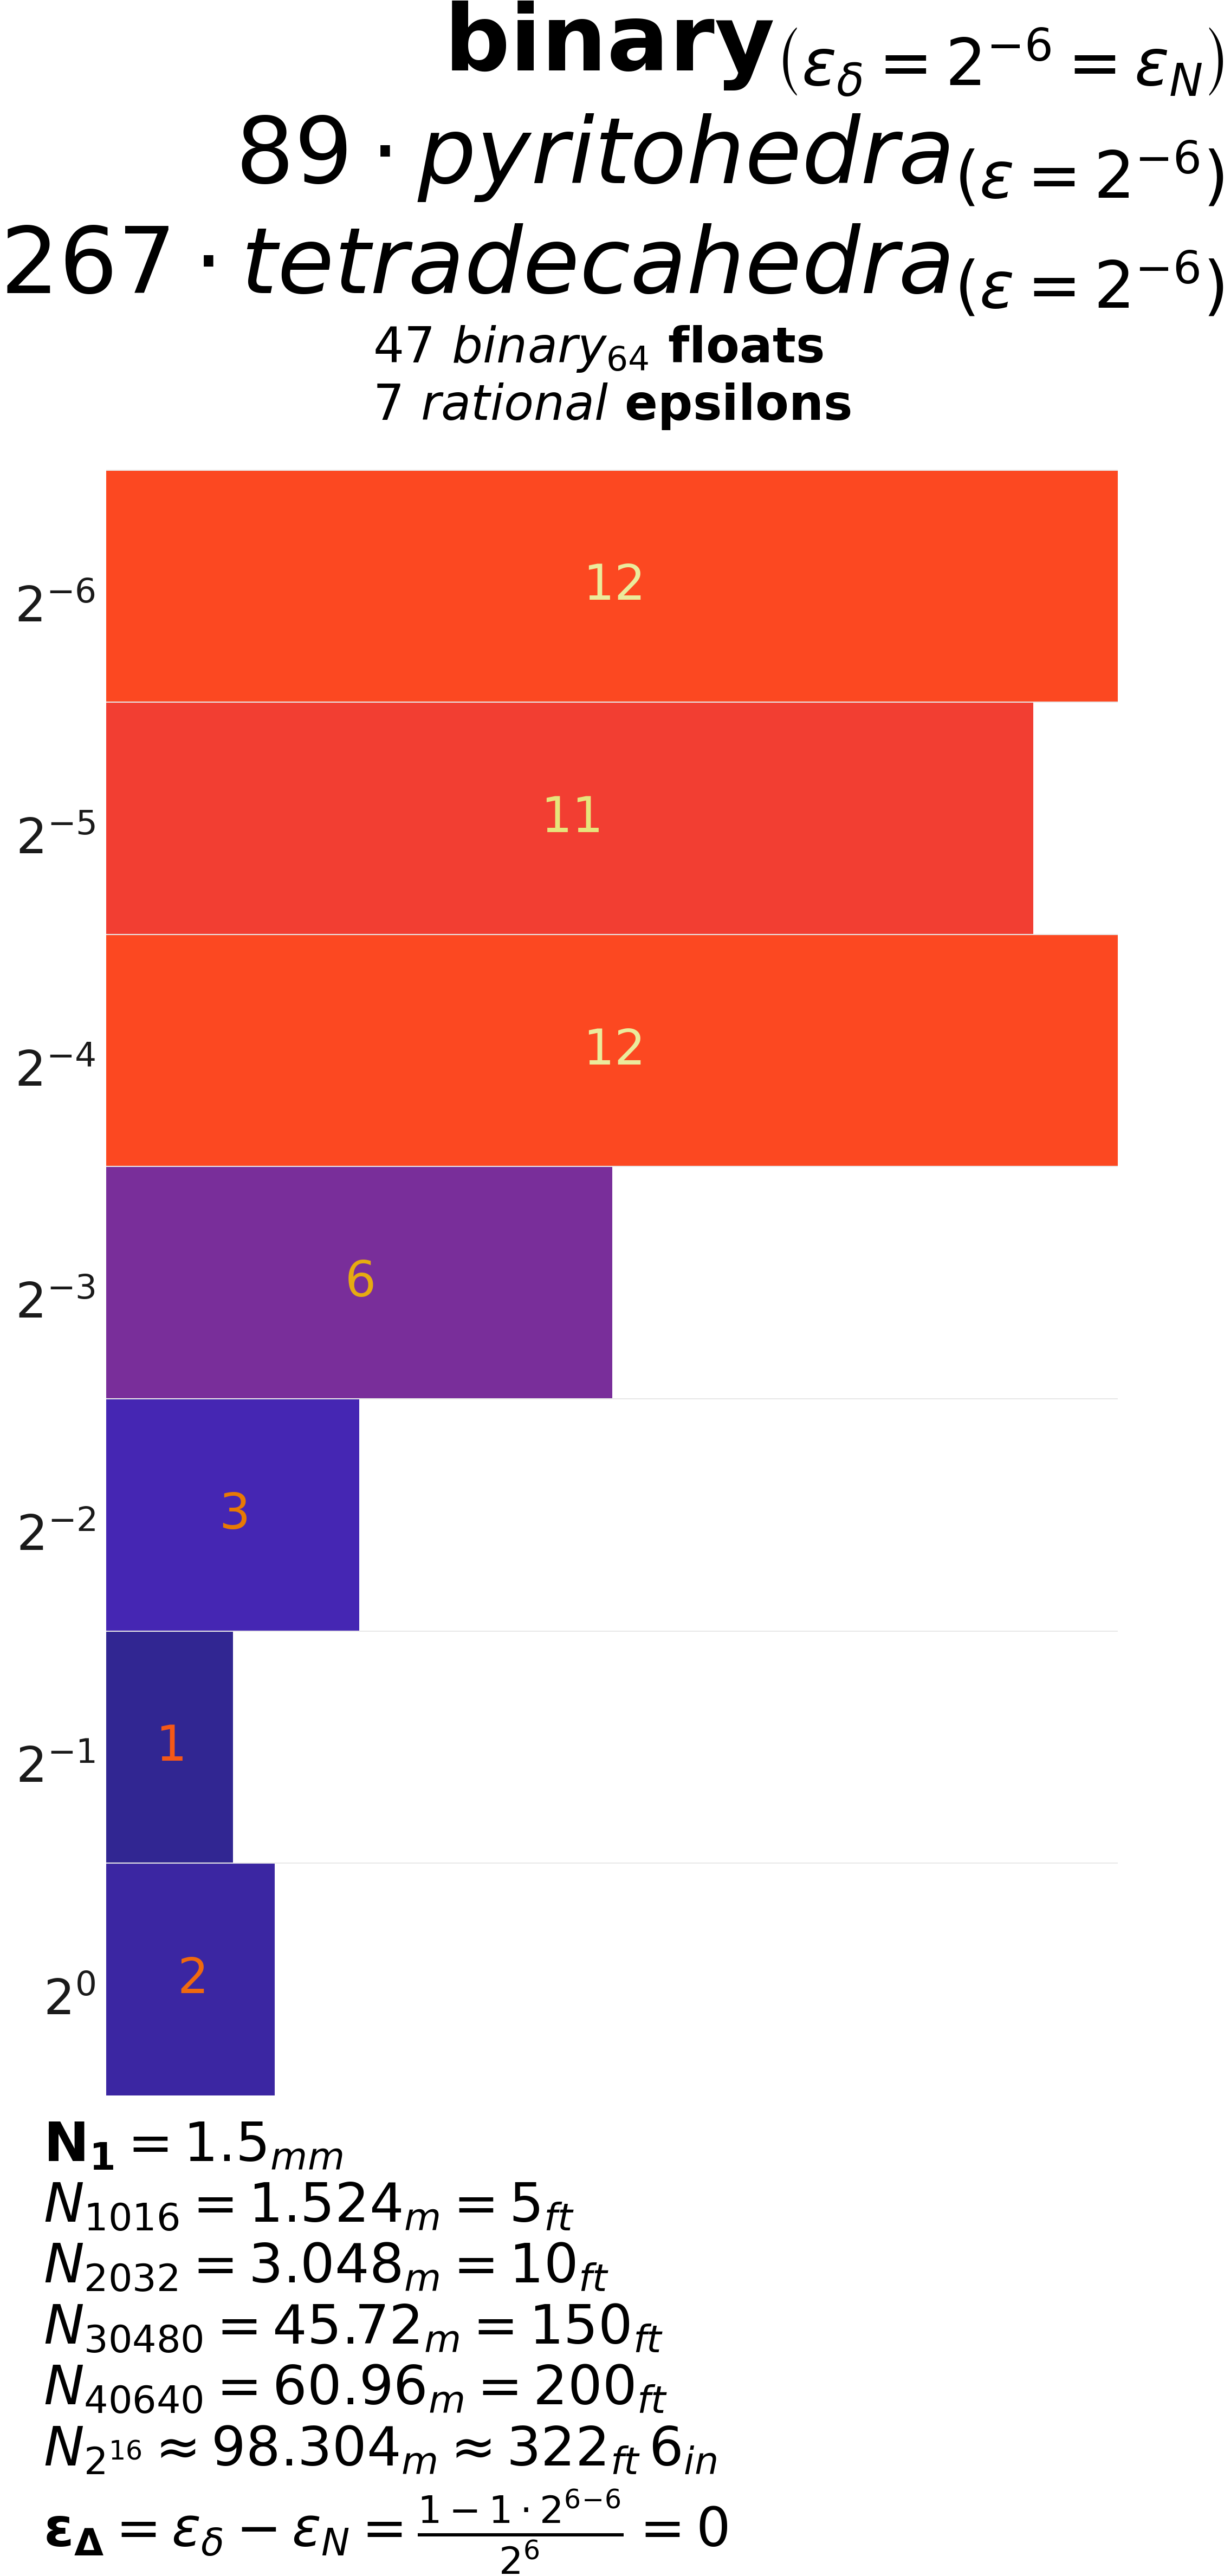
\includegraphics[width=.26\textwidth]{fig-histb}%
    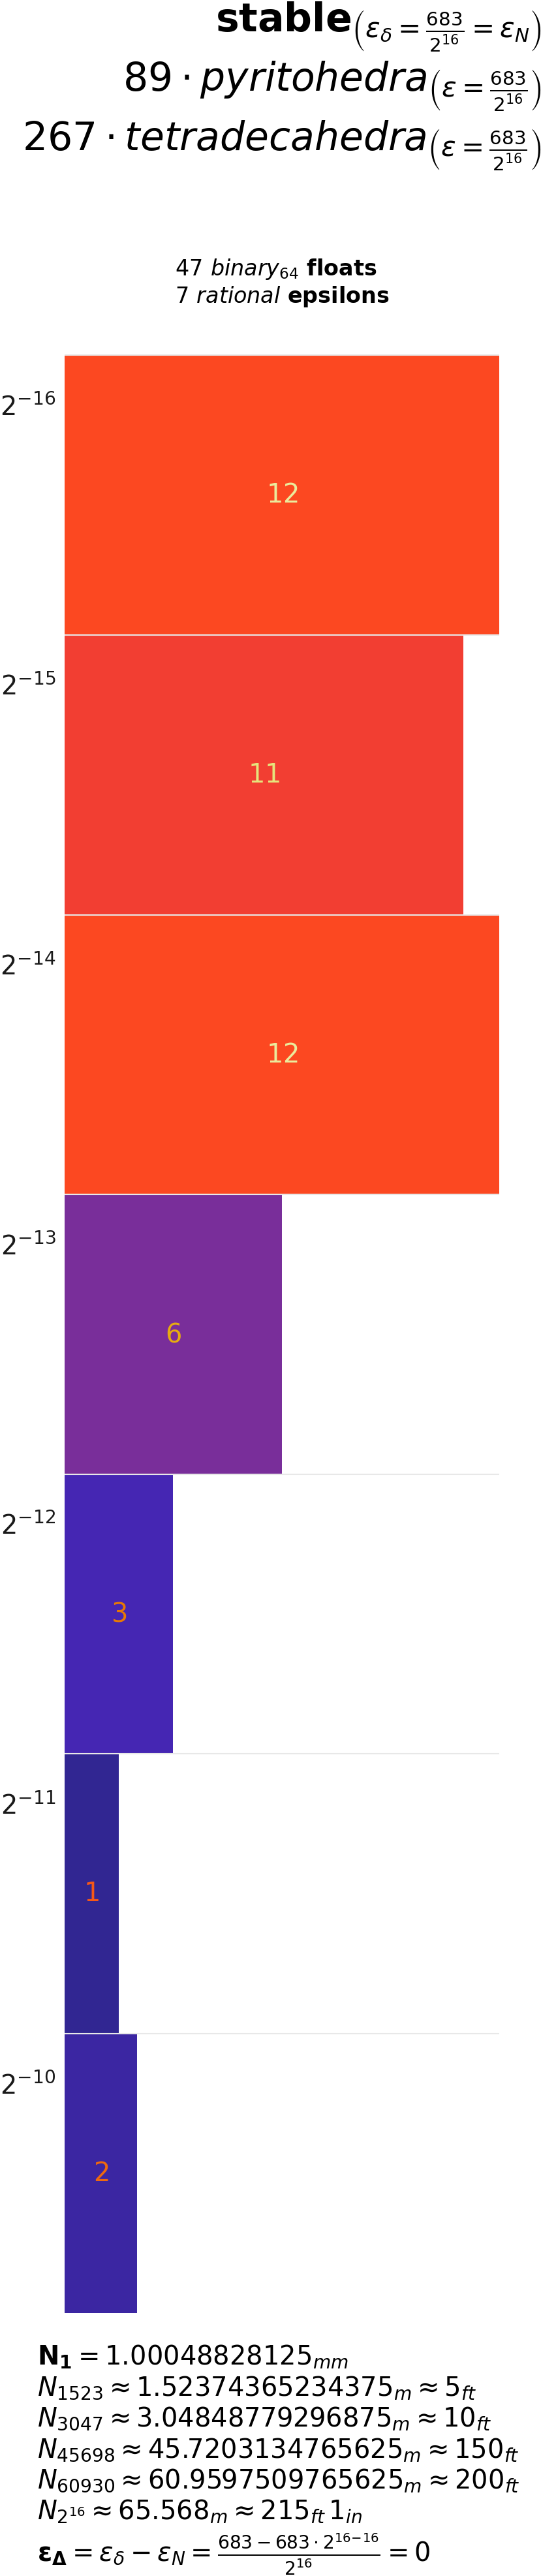
\includegraphics[width=.265\textwidth]{fig-hists}%
    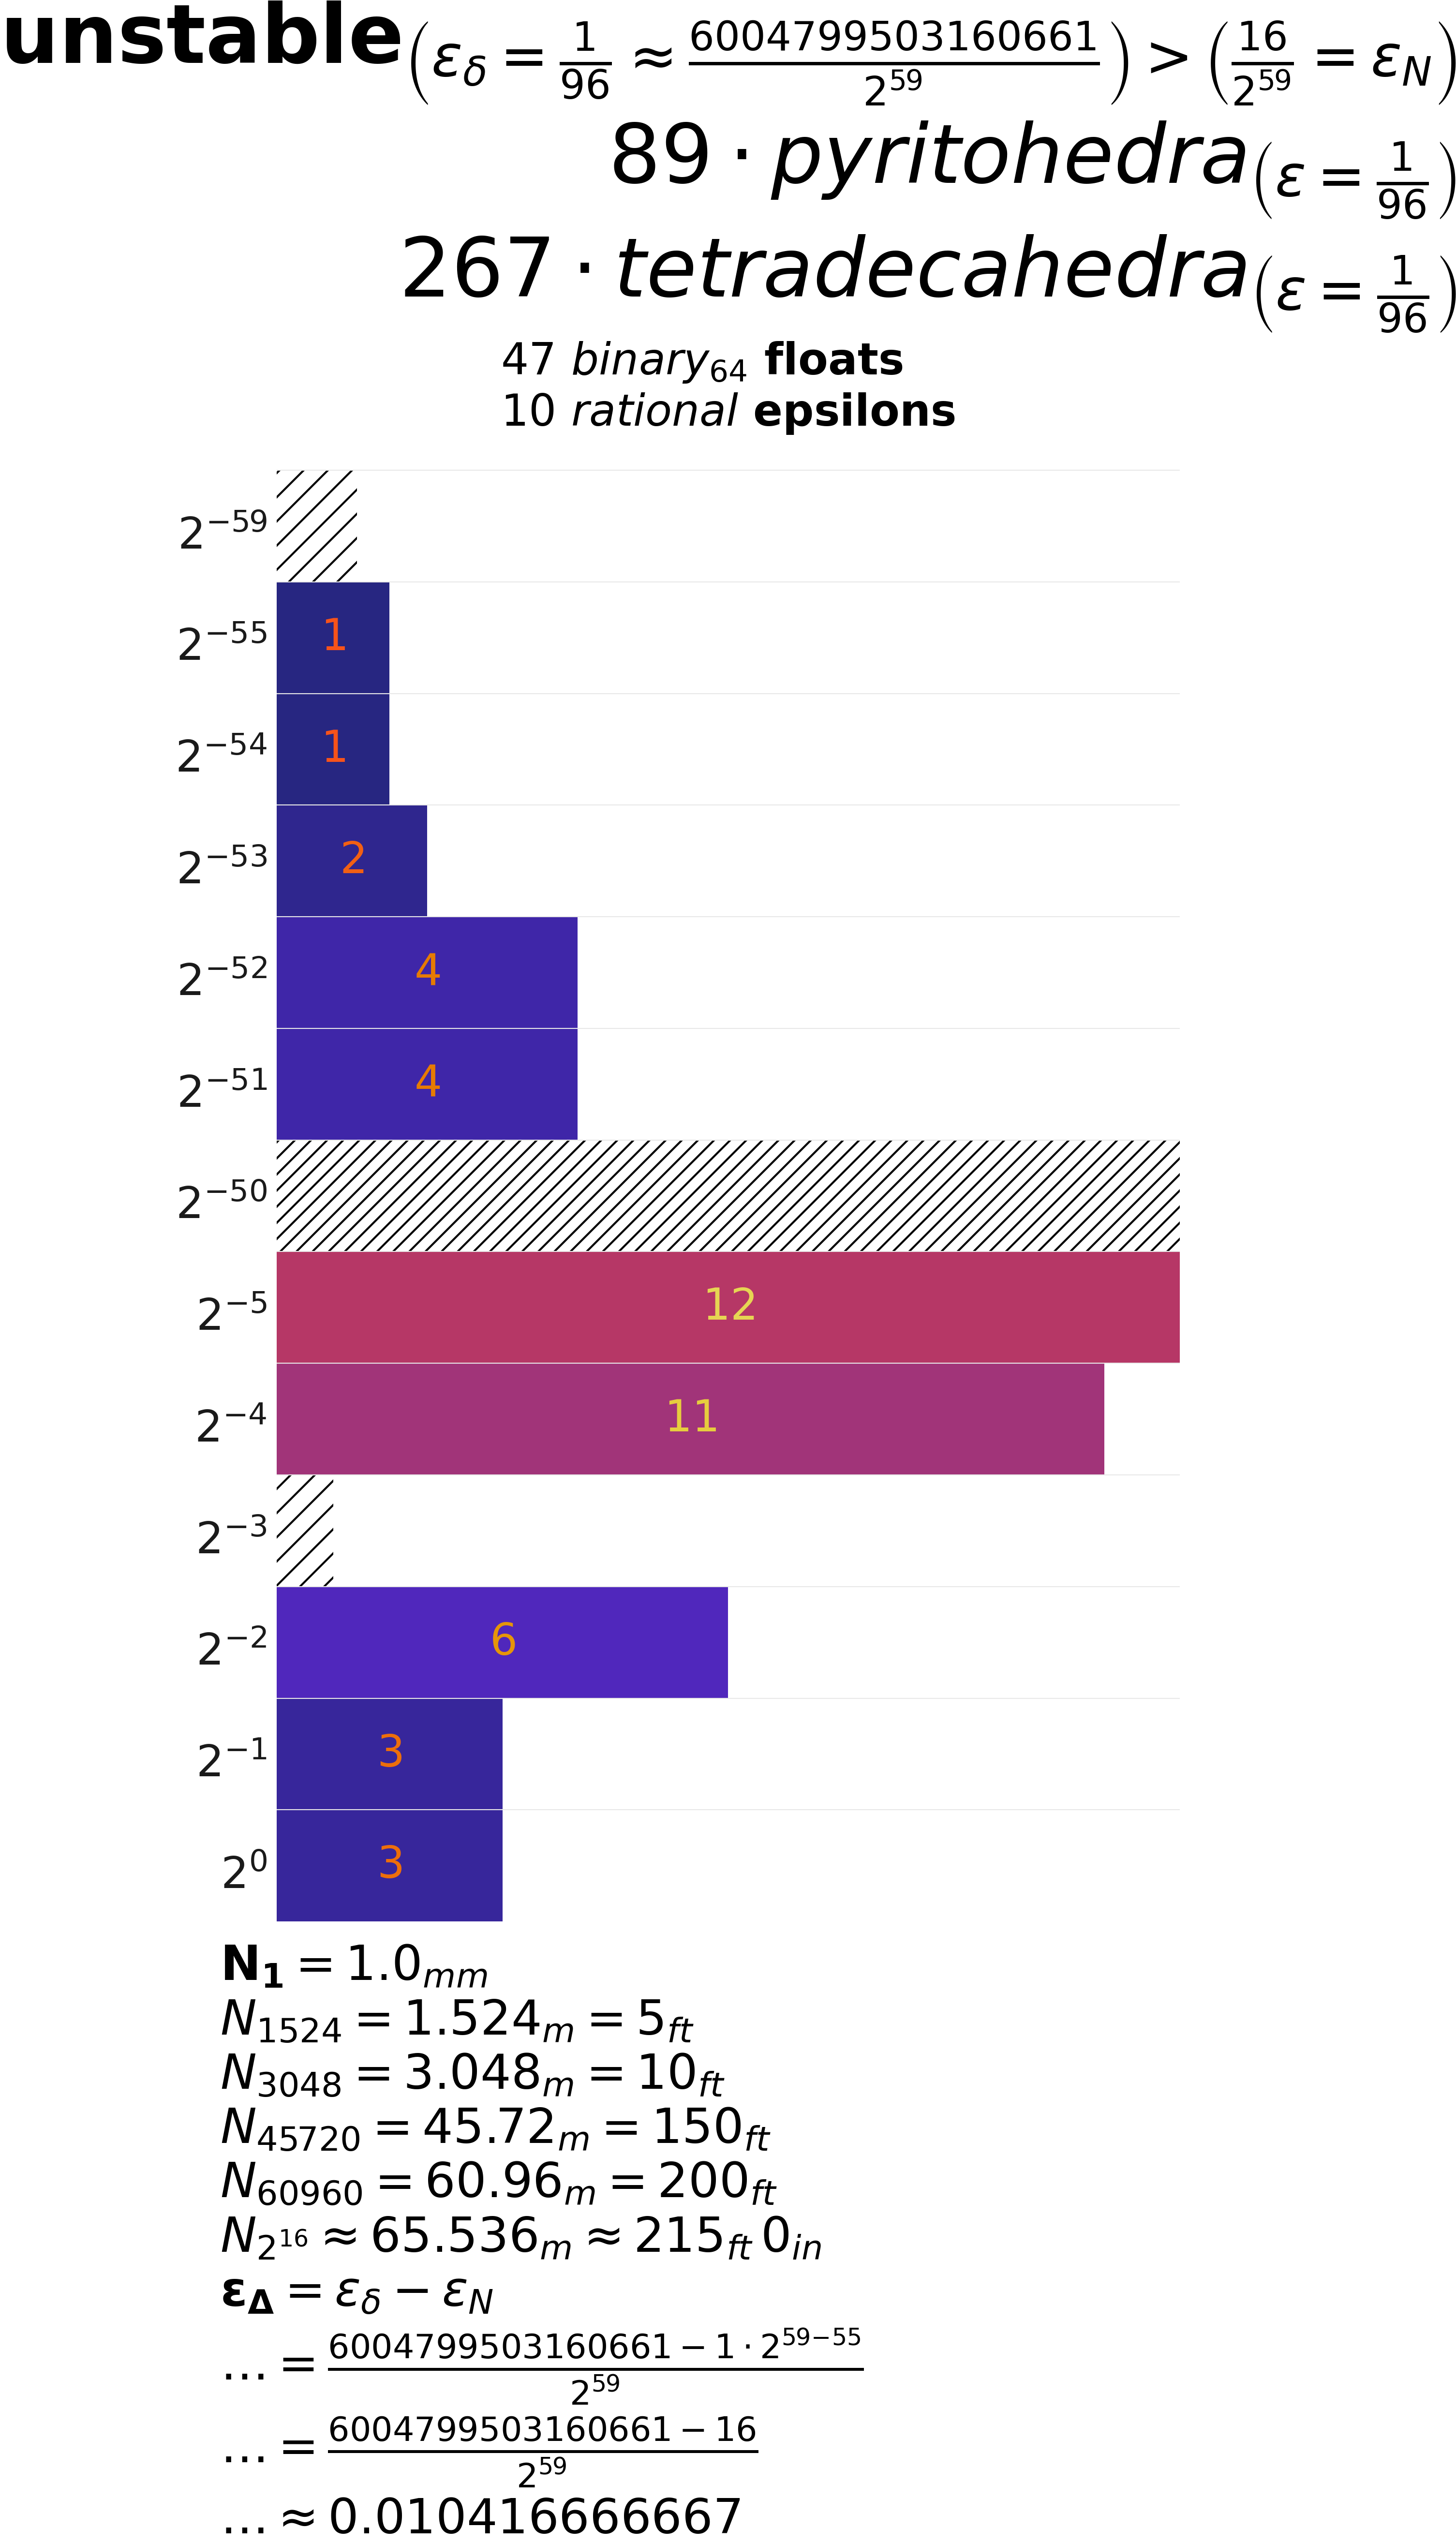
\includegraphics[width=.325\textwidth]{fig-histu}%
    \caption{Example histograms generated by \texttt{A15.py} (\texttt{-bars} option) illustrating numerical stability regimes for different output scaling factors ($\epsilon_\delta$). Left (\texttt{fig-histb.png.txt}, $\epsilon_\delta=1/64$): A \textbf{Binary} scale ($\epsilon_\Delta=0$) showing a single dominant denominator exponent ($n = \log_2 d$). Middle (\texttt{fig-hists.png.txt}, $\epsilon_\delta=683/2^{16}$): A \textbf{Stable} scale ($\epsilon_\Delta=0$) showing a contiguous block of exponents. Right (\texttt{fig-histu.png.txt}, $\epsilon_\delta=1/96$): An \textbf{Unstable} scale ($\epsilon_\Delta \neq 0$) showing a widely spread distribution with gaps, indicating floating-point approximation errors introduced during final scaling relative to the internal integer geometry.}
    \label{fig-hist}
\end{figure}

\subsection{\texttt{A15.py} Reference Implementation Overview}\label{subsec-implementation-a15py}

The Python script \texttt{A15.py} \cite{Risinger2024A15} serves as the reference implementation, exploratory tool, and validation instrument for the concepts presented in this research. It requires Python 3 and leverages standard scientific libraries—NumPy \cite{Harris2020} for efficient numerical array operations, SciPy \cite{Virtanen2020} for geometric computations (such as convex hull calculations used for visualization via \texttt{scipy.spatial.ConvexHull}), and Matplotlib \cite{Hunter2007} for versatile 2D and 3D visualization. The script's workflow systematically applies the principles of the \AAAB{} encoding framework, incorporating the crucial multi-stage scaling logic (\Cref{subsec-scaling-pipeline}) and the quantitative numerical stability analysis (\Cref{subsec-stability-validation}) described previously. \Cref{tab-a15py-workflow} summarizes the core stages of its operation, from parameter parsing to final visualization and validation. This structured process allows \texttt{A15.py} to generate, visualize, and analyze configurations, providing concrete examples and empirical validation of the framework's properties, such as the composite output shown in \Cref{fig-main}.

\begin{table}[!ht]
\centering
\caption{Core Workflow Stages in the \texttt{A15.py} Implementation.}
\label{tab-a15py-workflow}
\begin{tabularx}{\textwidth}{>{\raggedright\arraybackslash}p{0.18\textwidth} >{\raggedright\arraybackslash}X}
\toprule
\textbf{Stage} & \textbf{Key Functions \& Purpose in \texttt{A15.py}} \\
\midrule
Configuration Processing & \texttt{flags()}, \texttt{configuration()} \\
& Parses command-line arguments/files (\texttt{*.txt}). Interprets parameters (e.g., \texttt{scale}, \texttt{rescale}, \texttt{n}, \texttt{prescale}, \texttt{stix}, visualization flags like \texttt{-edges}, \texttt{-faces}, \texttt{-bars}). Handles defaults, automatic configurations (\texttt{-auto}), inheritance (colon notation). Determines final parameter set for generation and visualization. \\ \addlinespace
Shape Definition & \texttt{pyritohedron()}, \texttt{tetradecahedra()} \\
& Constructs fundamental geometric units based on parameters. Applies internal \texttt{prescale} factor converting base fractional coordinates to integer vertices relative to shape center. Handles local symmetry (handedness). \\ \addlinespace
Lattice Generation & \texttt{lattice()} \\
& Replicates shape units across 3D grid based on extent \texttt{n} and \texttt{at} filter (for basis site mapping). Calculates center positions using integer vectors \texttt{xyz}, origin offset \texttt{o}, and the fixed \texttt{* 24} spacing factor (relative to \texttt{prescale}d units), implicitly establishing the 96-unit effective baseline. Yields (vertex\_array, config\_object) pairs representing internal integer geometry. \\ \addlinespace
Scaling \& Stability Analysis & \texttt{figure()} \\
& Collects internal integer vertex arrays. Applies global \texttt{scale} parameter ($\epsilon_\delta$) mapping internal integers (relative to the 96-unit baseline) to output floats. Infers inherent base scale $\epsilon_N$. Calculates stability difference $\epsilon_\Delta$ (verifying if $\epsilon_\delta = m \cdot \epsilon_N$ for $m \in \mathbb{Z}^+ \implies \epsilon_\Delta=0$). \\ \addlinespace
Visualization \& Validation & \texttt{figure()} \\
& Renders 3D geometry via Matplotlib \cite{Hunter2007} using specified options (\texttt{-edges}, \texttt{-faces}, etc.). Uses SciPy \cite{Virtanen2020} for hull calculations if needed. If \texttt{-bars} requested, performs stability analysis (via \texttt{float.as\_integer\_ratio()} \cite{PythonDocsFloatRatio} denominators) and generates histogram (\Cref{fig-hist}), visualizing the stability regime and displaying $\epsilon_\Delta$. Outputs to screen (\texttt{-interactive} option implies pop-up) or file (\texttt{-savefig}). Includes annotations (\Cref{fig-main}). Relies heavily on NumPy \cite{Harris2020} throughout. \\
\bottomrule
\end{tabularx}
\end{table}

\begin{figure}[!htb]
    \capstart
    \centering
    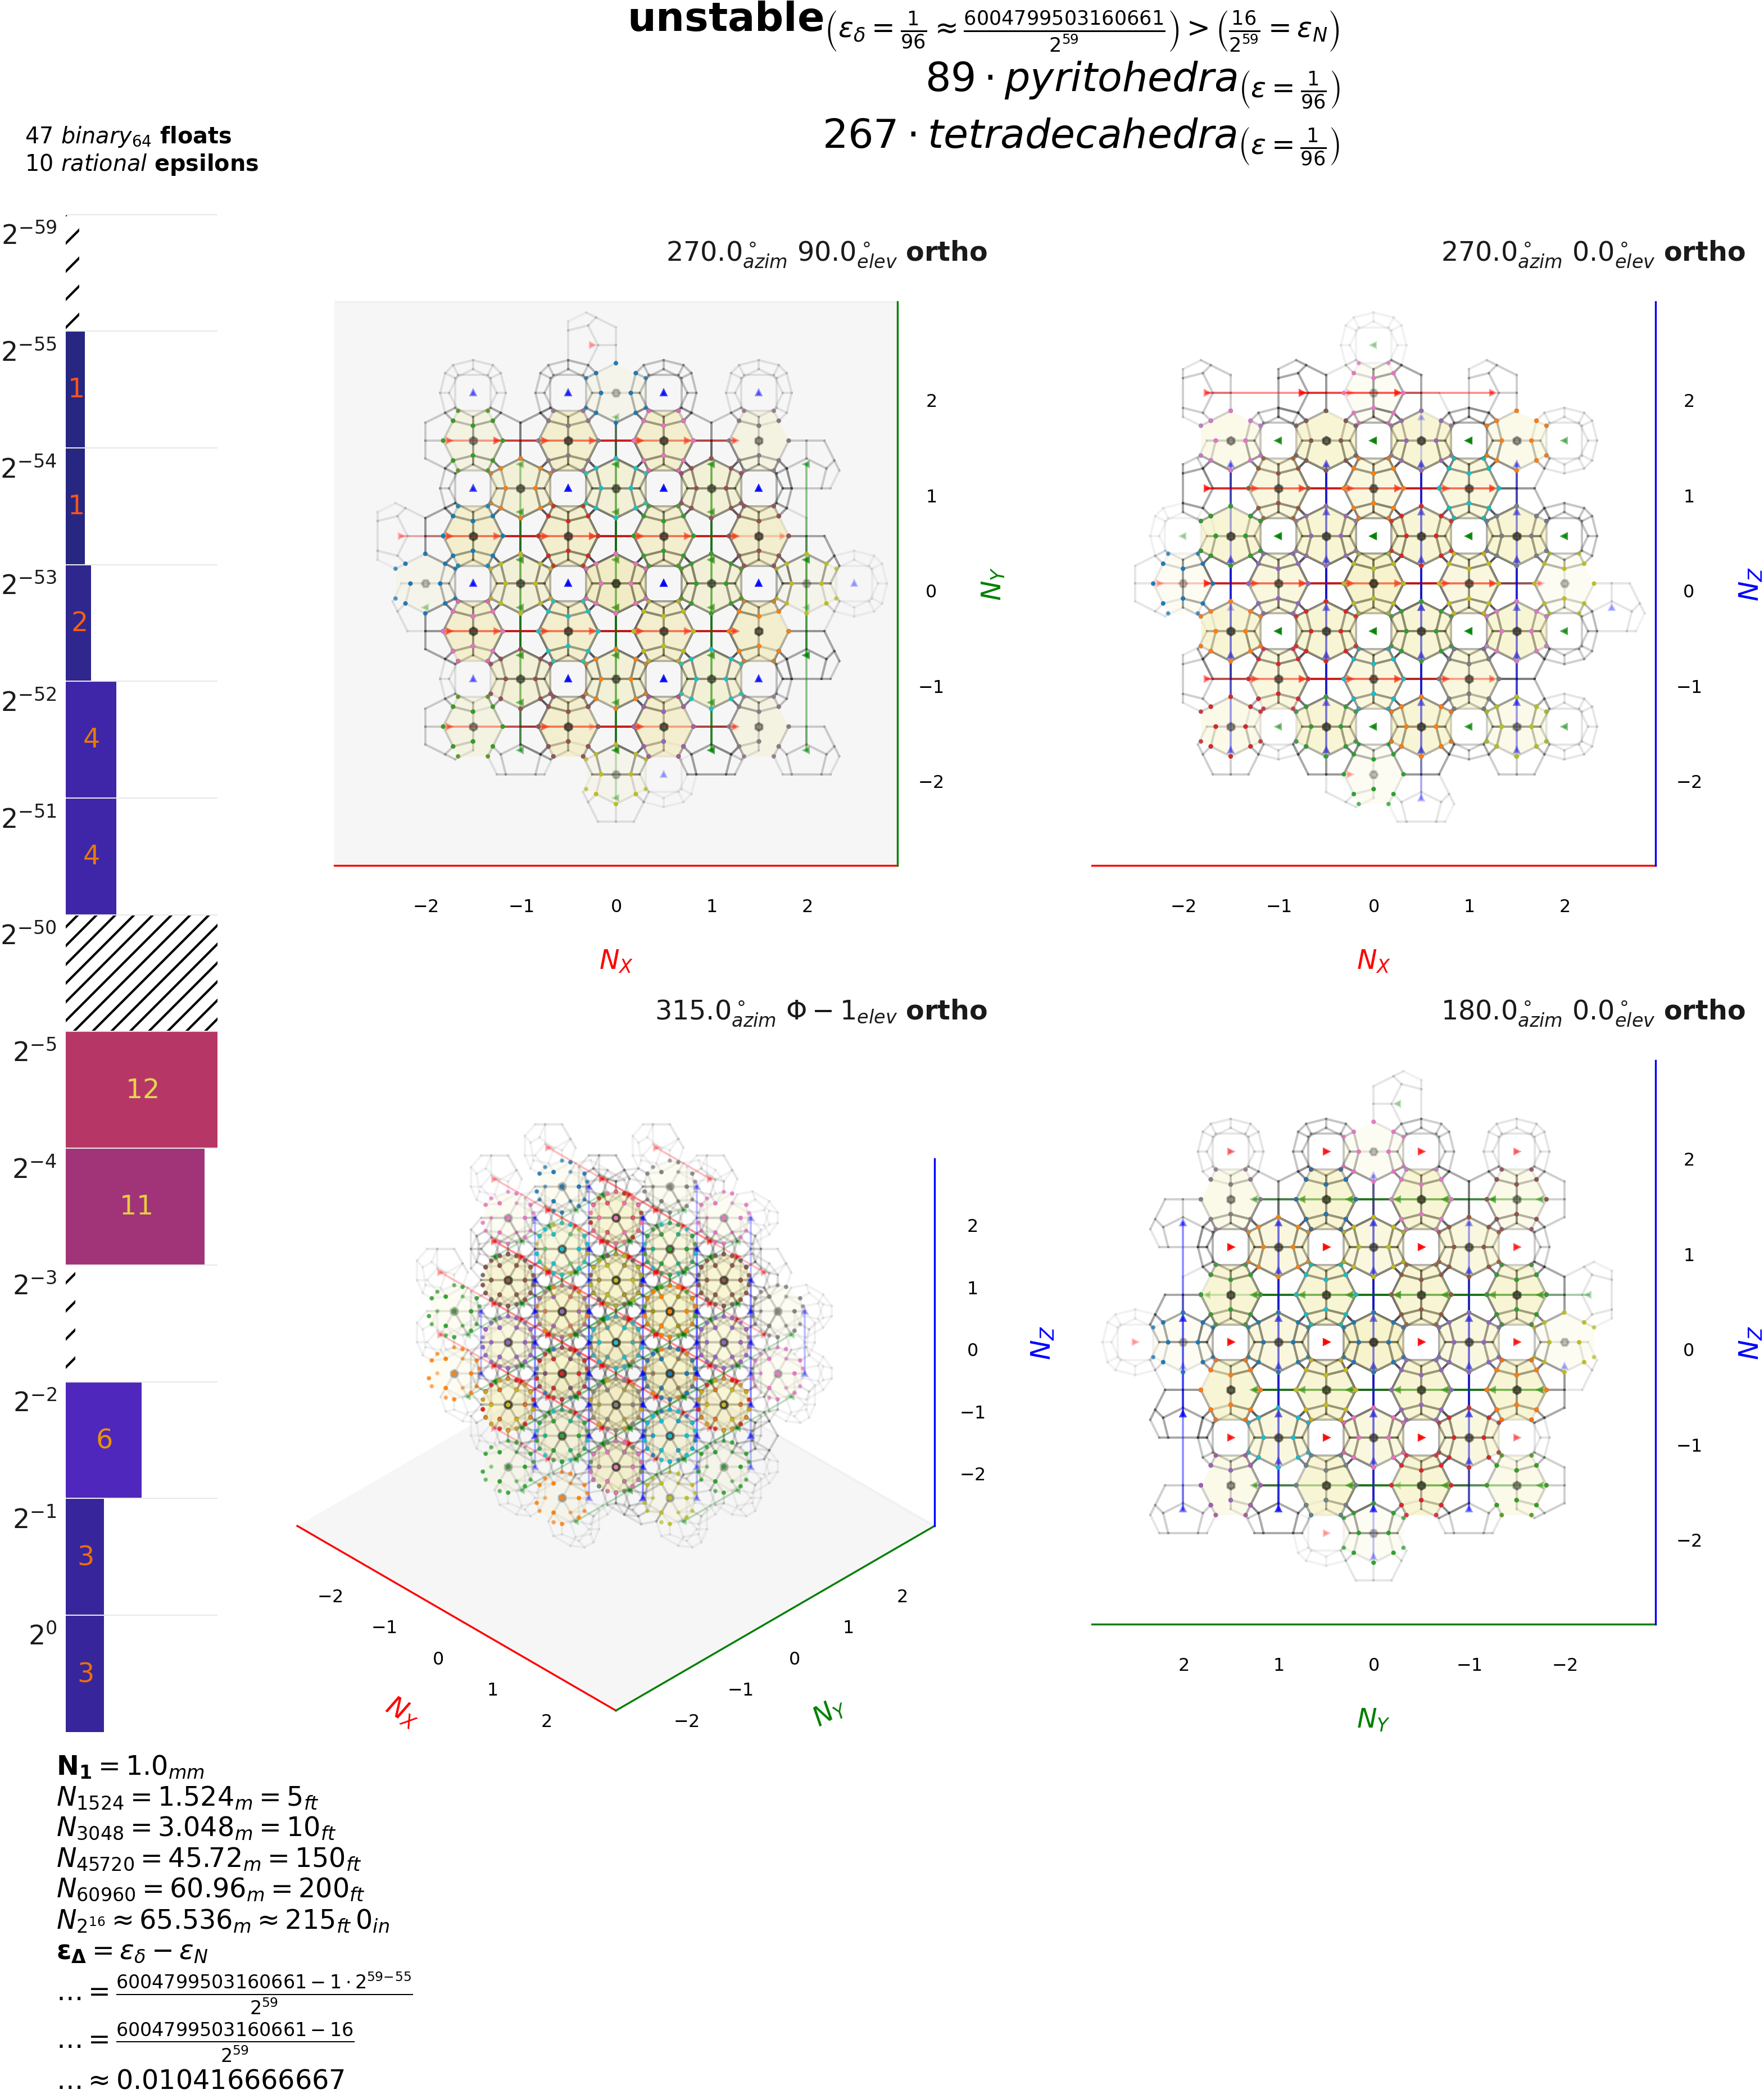
\includegraphics[width=0.8\textwidth]{fig-main}
    \caption{Composite visualization generated by \texttt{A15.py} (\texttt{fig-main.png.txt}) showing pyritohedra and tetradecahedra components alongside stability analysis. This example uses an \textbf{Unstable} output scale $\epsilon_\delta = 1/96$. The calculated non-zero stability difference ($\epsilon_\Delta \approx \num{0.0104} \neq 0$) is explicitly annotated in the histogram sidebar (left), confirming instability relative to the internal integer geometry. The histogram visually reflects this instability through its wide, gapped distribution of floating-point denominator exponents ($n = \log_2 d$). Main 3D views use dimensionless coordinates $N_X, N_Y, N_Z$ relative to the basic unit width $N_1$. For this specific unstable scale, $N_1$ corresponds to \SI{1.0}{\milli\meter}, derived from applying $\epsilon_\delta=1/96$ to the internal 96-unit effective lattice baseline. Counts shown refer to the number of float components analyzed for the histogram.}
    \label{fig-main}
\end{figure}

\section{Interpretation, Benefits, and Limitations}\label{sec-discussion}

The investigation detailed in the preceding sections confirms the distinctive suitability of the \AAAB{} phase structure, when employed within the numerically stable scaling framework (\Cref{sec-framework-design}), for partitioning interactive 3D spaces. The confluence of its inherent crystallographic properties (\Cref{sec-introduction}) and the demonstrable numerical stability achievable through disciplined scaling ($\epsilon_\Delta = 0$, \Cref{subsubsec-stability-diff}) yields a framework that is both geometrically sophisticated and computationally practical for demanding immersive applications. This section interprets these findings, highlights the quantifiable benefits derived directly from the framework's mechanics, and candidly discusses practical limitations and engineering considerations relevant to its implementation.

\subsection{Interpretation and Core Findings}\label{subsec-discussion-interpretation}

This research establishes \AAAB{} encoding as a robust structural foundation for coordinated spatial partitioning. The core finding is that by leveraging the specific crystallographic symmetries and binary-friendly coordinates of the \AAAB{} structure, and by rigorously adhering to the multi-stage scaling pipeline culminating in a stable output scale ($\epsilon_\Delta = 0$), it is possible to create a spatial representation that fundamentally eliminates floating-point representation errors relative to its own discrete grid. This provides a pathway to achieving verifiable determinism in spatial computations, a critical enabler for next-generation networked virtual environments and related spatial computing tasks.

\subsection{Quantifiable Benefits}\label{subsec-discussion-benefits}

The \AAAB{} encoding framework, when implemented correctly within stable scaling regimes, offers several key advantages validated by theoretical analysis and the \texttt{A15.py} \cite{Risinger2024A15} reference implementation:

\subsubsection{Guaranteed Determinism via Stable Scaling}\label{subsubsec-benefits-determinism}
Arguably the most significant contribution stems directly from operating within the rigorously defined \textbf{Binary} or \textbf{Stable} scaling regimes ($\epsilon_\Delta = 0$, \Cref{subsubsec-stability-regimes}). By precisely aligning the chosen output scale ($\epsilon_\delta$) with the structure's inherent geometric precision requirements ($\epsilon_N$, relative to the 96-unit baseline derived in \Cref{subsubsec-scaling-baseline}), the framework guarantees that all \AAAB{} lattice points and derived vertex coordinates map exactly onto hardware binary floating-point formats \emph{relative to that chosen stable scale}. This systematically eliminates the representation errors inherent in approximating arbitrary spatial positions with floats, at least within the context of the framework's quantized representation derived from the internal integer grid (\Cref{subsubsec-scaling-internal}). The result is guaranteed bit-level consistency and numerical determinism across disparate machines, platforms, and even different compilation environments—a fundamental prerequisite for reliable state synchronization in networked systems, reproducible physics simulations, efficient network delta compression strategies, verifiable event sequences and replays, and ultimately, fair and trustworthy competitive experiences.

\subsubsection{Memory and Bandwidth Efficiency}\label{subsubsec-benefits-efficiency}
Mapping continuous coordinates onto compact, often integer-based, \AAAB{} identifiers provides substantial memory and bandwidth savings compared to standard floating-point vector representations (\Cref{subsec-intro-floats}). This advantage is particularly pronounced when quantizing explicitly defined or bounded volumes where the full dynamic range and mantissa precision of standard floats represent unnecessary overhead. Storing or transmitting a 3D coordinate using a suitable \AAAB{}-based integer representation—for instance, a \SI{48}{\bit} integer capable of encoding both a vast cell index range and precise intra-cell positioning information—can reduce the data size by \textbf{50\% or more} compared to the \SI{96}{\bit} typically required for three standard single-precision (\SI{32}{\bit}) floats, as shown in \Cref{eq-efficiency-memory}.
\begin{equation} \label{eq-efficiency-memory}
    \text{Savings} = \frac{(96\,\text{bit} - 48\,\text{bit})}{96\,\text{bit}} \times 100\% = 50\%
\end{equation}
This efficiency translates directly into reduced memory footprints for spatial data structures and significantly lower network traffic for coordinate updates. Considering just baseline kinematic tracking data (\Cref{eq-bandwidth-baseline}), this reduction from approximately \SI{67.2}{\kilo\bit\per\second} down to \SI{34}{\kilo\bit\per\second} or less offers significant leverage on aggregate bandwidth, especially in complex scenarios often exceeding \SI{100}{\kilo\bit\per\second} per user for kinematics alone.
\begin{equation} \label{eq-bandwidth-baseline}
    \text{Rate}_{\text{3xFloat}} = 20\,\text{jts} \times (3_{\text{pos}} + 4_{\text{quat}})\,\tfrac{\text{floats}}{\text{jt}} \times 4\,\tfrac{\text{bytes}}{\text{float}} \times 15\,\text{Hz} = 8400\,\text{byte/s} \approx 67.2\,\text{kbit/s}
\end{equation}
The \AAAB{} integer encoding effectively reclaims storage and bandwidth otherwise consumed by unused float exponent bits and excess significand precision within suitably bounded contexts. Furthermore, this compactness and structural definition offer benefits for long-term data storage and archival, providing a potentially more stable and interpretable format compared to raw floating-point streams. Practical applications, such as the related \texttt{layoutc} project which encodes physical layouts using similar principles \cite{Risinger2024Layoutc}, demonstrate the utility of such compact, deterministic encodings.

\subsubsection{Geometric Fidelity and Isotropy}\label{subsubsec-benefits-geometry}
Leveraging the intrinsic crystallographic properties of the \AAAB{} structure (\Cref{subsec-intro-a15}) imparts beneficial geometric qualities to the spatial representation. Its verified high mean coordination number (13.5) indicates efficient local packing and dense connectivity between neighboring regions. The crucial $T_h$ point group symmetry provides a high degree of local isotropy by incorporating near-icosahedral geometric elements within a globally cubic (and thus perfectly periodic) framework (\Cref{subsec-intro-a15}). This structural integrity, especially when combined with the topologically matched \WPH{} local discretization method (\Cref{subsec-intro-partitioning}), fosters a spatially uniform or ``fair'' representation, helping to minimize the directional biases or artifacts that can plague simpler grid-based partitioning schemes.

\subsubsection{Suitability for Distributed Computing}\label{subsubsec-benefits-parallelism}
The inherent regularity, crystallographic symmetries, and predictable neighborhood topology of the A15 lattice provide a structured substrate well-suited for spatial domain decomposition. This facilitates the distribution of spatial computations across parallel architectures, including clusters, GPUs, or edge networks, potentially simplifying load balancing and data management compared to adaptive or irregular spatial structures. The deterministic nature of the grid ensures consistent partitioning across nodes operating under stable scaling regimes.

\subsubsection{Foundation for Enhanced Interoperability}\label{subsubsec-benefits-interoperability}
By establishing a common, mathematically precise, and verifiable spatial structure, the A15 framework offers a robust foundation for enhanced interoperability. Diverse applications adhering to the same A15 structure, scale, and orientation conventions could potentially exchange, reference, or merge spatial data with greater semantic consistency and reduced ambiguity, fostering cohesion across federated virtual environments or collaborative platforms.

\subsubsection{Validated Implementation Framework}\label{subsubsec-benefits-validation}
The accompanying \texttt{A15.py} script (\Cref{subsec-implementation-a15py}) serves as more than just a visualization aid; it is a validated reference implementation and analysis framework. It demonstrates the practical construction of \AAAB{}-based structures, rigorously implements the multi-stage scaling logic essential for achieving numerical stability (\Cref{subsec-scaling-pipeline}), and provides the quantitative histogram analysis (\Cref{subsec-stability-validation}, \Cref{fig-hist}) that empirically confirms the existence and accessibility of the stable scaling regimes ($\epsilon_\Delta = 0$). This ensures the reproducibility of the core findings regarding numerical stability and offers a concrete, verifiable starting point for developers seeking to implement or explore the \AAAB{} encoding framework for their own applications.

\subsection{Limitations and Engineering Considerations}\label{subsec-discussion-limits}

Despite its significant advantages for achieving determinism and efficiency, adopting the \AAAB{}-based partitioning approach involves several practical limitations and engineering challenges that require careful consideration during implementation. These represent addressable design aspects rather than fundamental flaws in the underlying concept:

\subsubsection{Complexity of Arbitrary Rotations}\label{subsubsec-limits-symmetry}
Applying arbitrary rotations *relative to the lattice axes* directly to the integer lattice coordinates used in \AAAB{} encoding can be intricate, particularly when mapping points onto valid \AAAB{} basis sites (Wyckoff 2a or 6d) or navigating complex cell boundaries like those in \tWPH{}. Correct implementation necessitates carefully calculated transformations aware of the crystal basis and space group operations \cite{ITCVolumeA2016}. However, the complexity is dependent on the nature of the rotation and the chosen local discretization method; axis-aligned rotations or operations within simpler partitioning geometries like \tTSP{} may present fewer complexities. Regardless of the approach, adopting a canonical orientation convention (\Cref{subsubsec-limits-handedness}) is essential for consistent interpretation and interoperability.

\subsubsection{Scalability and Spatial Federation}\label{subsubsec-limits-federation}
The framework naturally defines discrete, structured zones based on the generated \AAAB{} lattice extents (controlled by the \texttt{n} parameter in \texttt{A15.py}). Seamlessly extending this model to create massive, open-world environments requires robust mechanisms for managing transitions and maintaining coordinate and state consistency across the boundaries between independent \AAAB{} zones. Addressing this likely involves developing standardized inter-zone boundary protocols for coordinate transformations (potentially involving scale changes), object state hand-offs, and perhaps authority transfer between simulation domains. Level-of-Detail (LOD) systems \cite{Luebke2002} utilizing multi-resolution \AAAB{} grids (employing coarser quantization for distant or less critical zones, potentially via relative addressing) might also play a role in managing complexity at large scales.

\subsubsection{Quantization Cost and Design Alignment}\label{subsubsec-limits-quantization}
A practical consideration is the computational cost of quantization—mapping arbitrary continuous coordinates to the nearest discrete \AAAB{} identifier. While general-purpose nearest-neighbor searches in 3D can be computationally intensive, especially with complex cell boundaries (e.g., WPH), this cost is highly dependent on implementation strategy and application alignment. As noted (\Cref{subsec-scaling-framework}), if an application's coordinate system is deliberately aligned with a stable \AAAB{} scale ($\epsilon_\Delta = 0$), quantization can potentially become a highly efficient process dominated by integer arithmetic (e.g., truncation or bit shifts), making performance manageable through informed design choices rather than being an inherent bottleneck.

\subsubsection{Encoding Efficiency for Irregular Volumes}\label{subsubsec-limits-complex}
Using lattice-aligned cuboidal extents for defining \AAAB{} zones, while straightforward to implement via the \texttt{n} parameter, can lead to inefficient use of the addressable integer coordinate space when representing environments with highly irregular external boundaries, complex internal terrain features (like mountains or caves), or significant voids (e.g., the interior of large, non-rectangular buildings). This may result in significant portions of the allocated integer coordinate range being unused or unreachable within the playable or interactive space. Potential mitigations could include implementing secondary encoding or metadata schemes (e.g., run-length encoding of valid zones along axes, hierarchical spatial masks, sparse data structures like sparse voxel octrees adapted to the A15 lattice), exploring hybrid approaches that combine the regular \AAAB{} grid with adaptive structures primarily for managing boundary details or sparse areas (though this might reintroduce some complexity), or effectively managing precision and sparsity through hierarchical, multi-scale A15 grids utilizing relative addressing (\Cref{subsec-scaling-pipeline}).

\subsubsection{Distinction from Minimal Surface \WPH{}}\label{subsubsec-limits-wp-form}
It bears repeating that this research primarily utilizes the computationally tractable \emph{geometric polyhedral} form of the \WPH{} for local discretization (\Cref{subsec-intro-partitioning}). This form shares the essential topology and $Pm\bar{3}n$ symmetry with the A15 structure but is distinct from the theoretical, relaxed minimal-surface area structure associated with the Kelvin conjecture counter-example \cite{WeairePhelan1994}. Consequently, properties derived strictly from minimal surface studies (e.g., relating to precise surface tensions or the guarantee of absolutely equal cell volumes between the pyritohedral and tetradecahedral cells in the relaxed state \cite{Kusner1996}) do not necessarily translate directly to the geometric partitioning method employed here.

\subsubsection{Requirement for Handedness Convention}\label{subsubsec-limits-handedness}
While the overall $Pm\bar{3}n$ space group is centrosymmetric (achiral), the specific arrangement of atoms in the \AAAB{} structure's basis results in alternating left- and right-handed local coordination environments around the 6d sites (\Cref{subsec-intro-a15}). This local chirality is implemented deterministically based on lattice position within the \texttt{A15.py} reference code. However, for interoperability in any practical application, particularly networked ones, all participating systems \textbf{must establish and strictly adhere to a shared global orientation convention}. This convention dictates how these local chiralities are interpreted, represented, and transformed, ensuring consistency between different client implementations and, crucially, when interfacing with host environments or game engines that may use different native coordinate system handedness (e.g., left-handed systems common in Unity \cite{UnityCoords} and Unreal Engine \cite{UnrealCoords} versus right-handed systems standard in physics and mathematics). Without such a shared convention, mirrored or incorrectly oriented geometry could easily result from exchanging \AAAB{}-encoded coordinates.

\subsubsection{Privacy and Security of Tracking Data (PII)}\label{subsubsec-limits-privacy}
The application of this efficient encoding framework to fine-grained spatial tracking data, especially full-body kinematics derived from VR/AR systems, carries significant privacy implications that \textbf{must} be addressed with utmost seriousness. Such detailed movement data constitutes \textbf{Personally Identifiable Information (PII)} and may qualify as sensitive biometric data under various regulations (e.g., GDPR \cite{GDPR-2016}, CCPA \cite{CCPA-2018}). Handling this data demands rigorous privacy safeguards and unwavering ethical considerations as a \textbf{non-negotiable} aspect of implementation. Developers and deployers \textbf{must} integrate robust security measures as a foundational requirement. This includes, at a minimum:
\begin{itemize} \itemsep0pt
    \item Employing strong \textbf{end-to-end encryption (E2EE)} for all \AAAB{}-encoded coordinate streams and associated tracking data during network transmission and persistent storage.
    \item Strict adherence to \textbf{data minimization principles} (collecting only the data essential for the application's functionality).
    \item Implementing transparent \textbf{user consent mechanisms} before any tracking begins.
    \item Establishing clearly defined \textbf{data retention and deletion policies}.
    \item Utilizing effective \textbf{anonymization or aggregation strategies} whenever full individual fidelity is not strictly required (e.g., for analytics or heatmaps).
    \item Ensuring full compliance with all relevant legal and ethical regulations.
\end{itemize}
This data represents individuals and their behavior; it \textbf{must} be treated with the highest degree of care, respect, security, and transparency. Failure to do so carries significant legal, ethical, and reputational risks.

\section{Immediate Potential and Future Prospects}\label{sec-outlook}

The \AAAB{}-based spatial partitioning and encoding framework, validated for its numerical stability and efficiency (\Cref{sec-discussion}), offers immediate potential for enhancing current virtual environments and provides a solid foundation for future advancements in spatial computing. Its inherent structural and numerical properties lend themselves to broad applicability, while also opening intriguing avenues for further research and development aimed at refining and extending its capabilities.

\subsection{Immediate Practical Applications}\label{subsec-applications}

The practical adoption of \AAAB{} partitioning across diverse virtual platforms is facilitated by several key features, yielding tangible benefits for various applications available today:

\subsubsection{Cross-Platform Compatibility and Interoperability}\label{subsubsec-apps-coordsys}
The underlying $Pm\bar{3}n$ space group of the \AAAB{} structure is centrosymmetric, lacking inherent global chirality \cite{ITCVolumeA2016}. This structural property means the fundamental lattice encoding can be consistently represented within both \textbf{left-handed coordinate systems} (common in game engines like Unity \cite{UnityCoords} and Unreal Engine \cite{UnrealCoords}) and \textbf{right-handed systems} (standard in mathematics and physics) through straightforward external affine transformations. While this simplifies cross-platform integration, achieving unambiguous interoperability absolutely requires establishing and adhering to a shared global orientation convention (\Cref{subsubsec-limits-handedness}). Crucially, the shared mathematical foundation provides a pathway toward application-agnostic spatial understanding, enabling potentially more seamless data exchange between disparate systems built upon the same A15 conventions.

\subsubsection{Alignment with Global Measurement Standards}\label{subsubsec-apps-measurement}
The explicit output scaling mechanism ($\epsilon_\delta$, controlled via the \texttt{-scale} parameter in \texttt{A15.py}) allows the dimensionless internal \AAAB{} lattice coordinates (relative to the 96-unit effective baseline, \Cref{subsubsec-scaling-baseline}) to map directly and predictably onto standard physical units, such as SI meters or Imperial feet. Critically, selecting a scale factor within the Binary or Stable regimes ($\epsilon_\Delta=0$, \Cref{subsubsec-stability-regimes}) ensures this mapping is exact relative to the framework's chosen resolution. This facilitates interoperability not only between virtual systems but also with real-world measurements, enhancing user comprehension and grounding virtual spaces in familiar metrics. For instance, the recommended baseline scale of $\epsilon_\delta = 2^{-6}$ (\texttt{-scale=1/64}) provides robust sub-millimeter precision while operating within a numerically stable regime, yielding a basic unit width ($N_1$) of \SI{1.5}{\milli\meter} (\Cref{subsubsec-notes-figures}), suitable for many human-scale interactions.

\subsubsection{Foundation for Networked and Distributed Systems}\label{subsubsec-apps-network}
As established (\Cref{subsubsec-benefits-efficiency}, \Cref{subsubsec-benefits-determinism}), the combination of compact integer-based representation and guaranteed coordinate consistency achieved within stable scaling regimes ($\epsilon_\Delta = 0$) is arguably the framework's most crucial advantage for networked systems. It significantly reduces bandwidth requirements, especially for high-frequency data like kinematic tracking (\Cref{eq-bandwidth-baseline}), while providing an essential foundation for reliable state synchronization. This enables more efficient network delta compression, consistent physics interactions, verifiable command processing, and robust replay capabilities—all vital for fair, coherent, and maintainable shared virtual experiences. Furthermore, the regular, predictable structure provides a substrate amenable to efficient spatial partitioning for distributed computation across parallel architectures (clusters, GPUs, edge networks), simplifying domain decomposition and potentially improving load balancing (\Cref{subsubsec-benefits-parallelism}).

\subsubsection{Hierarchical Representation via Relative Addressing}\label{subsubsec-apps-relative}
The framework naturally enables multi-scale representations through relative addressing (\Cref{subsec-scaling-pipeline}). Applications can utilize this capability to encode coarse global positions efficiently while representing fine-grained local details (like avatar kinematics or intricate environmental features) with high precision relative to a parent coordinate. For example, an avatar's core position could be stored on a moderate-resolution A15 grid, while its complex joint movements are encoded on a much finer A15 grid defined locally relative to that core position. This approach optimizes the balance between data size, spatial range, and the level of detail required for different components of a scene.

\subsubsection{Implicit Spatial Constraints}\label{subsubsec-apps-constraints}
Mapping potentially vast continuous space onto the finite set of coordinates defined by the \AAAB{} partitioning inherently establishes the boundaries of the addressable virtual space for a given zone and scale. This acts as a passive, built-in mechanism for enforcing spatial limits. It can naturally prevent certain classes of common exploits involving out-of-bounds positioning and may simplify application logic required for validating entity positions relative to the defined interactive space, especially compared to managing complex boundary conditions in a purely floating-point environment.

\subsubsection{Potential for Computation Optimization}\label{subsubsec-apps-optimization}
Beyond memory savings and distribution benefits, the regular lattice structure enables integer-based addressing and highly predictable neighbor relationships. This regularity could potentially be leveraged for optimized spatial query algorithms (e.g., proximity searches, ray casting within the lattice using integer arithmetic) compared to navigating complex adaptive tree structures common in traditional spatial indexing (\Cref{subsec-comparison-indexing}). Particularly, if applications align their coordinate systems with a stable A15 scale, quantization and potentially other spatial operations might reduce to highly efficient integer math (\Cref{subsubsec-limits-quantization}), offering significant computational performance benefits in certain scenarios. Furthermore, in scenarios utilizing hierarchical representations with relative scaling (\Cref{subsubsec-apps-relative}), especially where scaling factors are powers of two (common in level-of-detail schemes), there may be opportunities to implement scaling directly via floating-point exponent manipulation, potentially offering further performance gains, although careful validation is essential to ensure such low-level operations maintain the integrity and deterministic guarantees of the A15 framework's coordinate mapping. Further investigation and benchmarking are needed to quantify these potential gains.

\subsubsection{Exemplar Use Cases}\label{subsubsec-apps-usecases}
These features position \AAAB{} partitioning as a robust foundation suitable \emph{now} for demanding applications. Examples include: competitive multiplayer VR esports requiring fairness and low latency; industrial digital twins demanding precise spatial fidelity and deterministic simulation; large-scale distributed physics or agent-based simulations needing reliable state consistency; collaborative mixed-reality (MR) systems requiring shared spatial understanding across diverse devices; and procedural content generation systems benefiting from deterministic spatial addressing. The related \texttt{layoutc} project, encoding physical layouts \cite{Risinger2024Layoutc}, provides a concrete example of applying similar compact, deterministic principles in practice.

\subsection{Future Research Directions}\label{subsec-outlook-research}

The \AAAB{} partitioning framework, while demonstrating immediate utility, also catalyzes numerous avenues for future research aimed at further enhancing immersive experiences and extending the capabilities of spatial computing:

\subsubsection{AI and Machine Learning Integration}\label{subsubsec-outlook-ai-ml}
The structured, high-fidelity, and deterministic spatial data encoded via \AAAB{} could provide a superior substrate for training artificial intelligence (AI) agents (e.g., non-player characters (NPCs), physics predictors, behavioral models). A consistent spatial representation might reduce environmental noise and improve learning efficiency for tasks involving complex spatial reasoning, navigation, pathfinding, prediction, and interaction within precisely defined virtual environments.

\subsubsection{Metaverse Interoperability Protocols}\label{subsubsec-outlook-interop}
Standardized protocols built upon \AAAB{} encoding (or similar deterministic lattice-based systems) could define universal mechanisms for agent state representation, coordinate referencing, interaction semantics, and capability negotiation across different \AAAB{}-partitioned virtual spaces or worlds, leveraging the common structural foundation discussed in \Cref{subsubsec-benefits-interoperability}. This could enable seamless transitions between independently managed environments, facilitate dynamic federation of spaces (\Cref{subsubsec-limits-federation}), and provide consistent object or avatar referencing across a heterogeneous metaverse built on deterministic spatial principles.

\subsubsection{Lattice Optimization and Alignment}\label{subsubsec-outlook-lattice}
Further investigation could explore the performance or perceptual benefits of aligning specific \AAAB{} crystallographic directions (e.g., high-density directions like $\langle 111 \rangle$ or $\langle 100 \rangle$) with dominant axes of expected user movement or interaction within particular virtual environment designs. Such alignment might yield computational performance gains (e.g., improved cache locality for neighborhood queries, simpler quantization logic as per \Cref{subsubsec-limits-quantization}) or perceptual benefits (e.g., reduced spatial aliasing effects along common traversal paths).

\subsubsection{Advanced Complex Geometry Representation}\label{subsubsec-outlook-complex}
Developing robust and efficient methods for representing non-cuboid volumes or complex geometric features within the A15 framework (\Cref{subsubsec-limits-complex}) remains a key area for practical improvement. Research could explore hybrid approaches combining the base A15 grid with techniques like sparse octrees or boundary representations for detail, investigate constructive solid geometry (CSG) operations defined relative to A15 cells, or further develop multi-resolution \AAAB{} representations (spatial Level-of-Detail, LOD \cite{Luebke2002}) perhaps utilizing the framework's inherent support for relative addressing (\Cref{subsubsec-apps-relative}) to handle varying levels of detail across large or intricate spaces more effectively.

\subsubsection{Exploration of Alternative Geometric Structures}\label{subsubsec-outlook-geometry}
While A15 offers a compelling balance of properties derived from crystallography, exploration of alternative partitioning or encoding schemes derived from related or more exotic mathematical structures could yield novel insights or properties advantageous for specific applications. Areas for investigation include:
\begin{itemize} \itemsep0pt
    \item \textbf{Triply Periodic Minimal Surfaces (TPMS):} Structures like the Gyroid \cite{Schoen1970} possess complex topology useful for flow simulation or intricate environment design, likely requiring implicit surface representations.
    \item \textbf{Quasicrystalline Patterns:} Non-periodic tilings exhibiting symmetries forbidden in periodic crystals (like 5-fold rotation \cite{Shechtman1984}) could enable partitioning schemes with unique tiling properties or isotropy characteristics.
    \item \textbf{Optimized Point Sets (e.g., Delone Sets):} Computationally generated point distributions balancing criteria like density and minimum separation guarantees \cite{Gruber2007} could tailor partitioning more closely to specific application requirements than regular lattices.
    \item \textbf{Higher-Dimensional Projections:} Projecting regular polytopes or honeycombs (e.g., from 4D \cite{Coxeter1973}) can generate novel 3D structures with useful partitioning properties.
\end{itemize}

\subsubsection{Perceptual and Cognitive Impact Studies}\label{subsubsec-outlook-perception}
Interdisciplinary research involving human-computer interaction (HCI) and cognitive science is needed to investigate how the specific geometric properties of different underlying spatial partitioning schemes (e.g., \AAAB{} or \WPH{} vs. simpler grids) affect human spatial perception, navigation efficiency, wayfinding accuracy, cognitive load, and the subjective sense of presence or realism within virtual environments. Such studies could provide valuable empirical data for human-centered design of virtual spaces.

\vspace{\parskip}
Pursuing these directions promises to expand the capabilities of structurally informed spatial partitioning. The intersection of crystallographic principles, computational geometry, numerical analysis, and real-time interactive systems represents a fertile territory for extending beyond entertainment into scientific visualization, collaborative design, distributed simulation, robotics, and the broader architecture of spatial computing itself.

\section{Supplementary Information}\label{sec-supplementary}

This section provides guidelines for replicating the results presented using the accompanying code, details supplementary resources available online, and discusses additional technical considerations relevant to the implementation and interpretation of the \AAAB{} encoding framework.

\subsection{Code Availability and Replication Protocols}\label{subsec-replication}

The figures and structural data presented in this research were generated using the accompanying Python script, \texttt{A15.py} \cite{Risinger2024A15}, which serves as the reference implementation. To ensure reproducibility, users should have Python 3 installed along with the standard scientific libraries NumPy \cite{Harris2020}, SciPy \cite{Virtanen2020}, and Matplotlib \cite{Hunter2007}. Understanding the script's execution flow (\Cref{tab-a15py-workflow}) and key parameters, particularly those governing the multi-stage scaling framework (\Cref{subsec-scaling-pipeline}) and numerical stability validation (\Cref{subsec-stability-validation}), is essential for proper use and interpretation of results.

The core Python script (\texttt{A15.py}), configuration files (\texttt{*.png.txt}) used for figure generation, the LaTeX source for this manuscript (or a version thereof), and extended documentation are publicly available within the \IL{} \texttt{space} repository on GitHub \cite{InfimaSpace}:
\begin{center}
    \url{https://github.com/infimalabs/space/tree/main/A15}
\end{center}
A project overview and supplementary materials may also be found at the project's homepage:
\begin{center}
    \url{https://infima.space/A15/}
\end{center}
The related project \texttt{layoutc}, applying similar compact encoding concepts to paintball field layouts \cite{Risinger2024Layoutc}, is also available via associated repositories:
\begin{center}
    \url{https://github.com/infimalabs/layoutc}
\end{center}

Achieving deterministic results, a core goal of this framework, relies crucially on operating within the \textbf{Binary} or \textbf{Stable} scaling regimes ($\epsilon_\Delta = 0$, \Cref{subsubsec-stability-regimes}). The recommended baseline scale of $\epsilon_\delta = 2^{-6}$ (\texttt{-scale=1/64}) generally provides a practical balance for human-scale interactions, offering high precision (approximately \SI{1.5}{\milli\meter} basic unit width $N_1$, see \Cref{subsubsec-apps-measurement} and \Cref{subsubsec-notes-figures}) while ensuring exact floating-point representability relative to the internal grid for typical configurations. Users are strongly encouraged to employ the \texttt{-bars} analysis feature (\Cref{subsec-stability-validation}) to explicitly verify the stability ($\epsilon_\Delta = 0$) of any custom configurations before deployment in applications where determinism is critical.

Furthermore, while \texttt{A15.py} deterministically implements alternating handedness for local coordination environments based on lattice position (\Cref{subsubsec-limits-handedness}), networked applications or systems exchanging \AAAB{}-encoded data \textbf{must} establish and consistently apply a shared global orientation convention to ensure interoperability and prevent geometric mirroring between different clients or system components.

\subsubsection{Example Replication Commands}\label{subsubsec-repl-commands}
The primary figures presented in this manuscript can be regenerated using the \texttt{A15.py} script and the corresponding configuration files (typically named \texttt{fig-\textit{name}.png.txt}) provided in the supplementary materials repository (\Cref{subsec-replication}). Ensure the script and configuration files are accessible in the execution environment. Use the \texttt{-i} (or \texttt{-pop}) option for interactive viewing (requires a graphical display environment):

\begin{description} \itemsep0pt
    \item[\Cref{fig-intro} (Intro):] Nested \AAAB{} (Multiple Scales) \\
        \texttt{python3 A15.py -i fig-intro.png.txt}
    \item[\Cref{fig-cell2} (Internals):] Left-Handed $^1/_2$ Unit Cell \\
        \texttt{python3 A15.py -i fig-cell2.png.txt}
    \item[\Cref{fig-wp-ts} (Partitions):] \WPH{} and \TSP{} \\
        \texttt{python3 A15.py -i fig-wp.png.txt} \\
        \texttt{python3 A15.py -i fig-ts.png.txt}
    \item[\Cref{fig-main} (Composite):] Representative Example (Unstable Scale) \\
        \texttt{python3 A15.py -i fig-main.png.txt}
    \item[\Cref{fig-hist} (Histograms):] Binary, Stable, and Unstable Scales \\
        \texttt{python3 A15.py -i fig-histb.png.txt} \\
        \texttt{python3 A15.py -i fig-hists.png.txt} \\
        \texttt{python3 A15.py -i fig-histu.png.txt}
\end{description}
For a detailed explanation of all command-line options, parameters, configuration file syntax, and advanced usage, refer to \texttt{python3 A15.py --help}.

\subsection{Supporting Notes and Clarifications}\label{subsec-supplementary-notes}

Further details, data, and clarifications related to this research are provided below.

\subsubsection{Bandwidth Calculation Basis}\label{subsubsec-notes-bandwidth}
The discussion regarding network bandwidth requirements (\Cref{subsubsec-benefits-efficiency}, \Cref{subsubsec-apps-network}) utilizes a baseline calculation (\Cref{eq-bandwidth-baseline}) assuming a single avatar with 20 tracked joints, each transmitting 3D position (3x \SI{32}{\bit} floats) and an orientation quaternion (4x \SI{32}{\bit} floats) at a \SI{15}{\hertz} update rate (\approx \SI{67.2}{\kilo\bit\per\second}). This kinematic component typically represents only a fraction of the total network traffic in complex interactive applications.

\subsubsection{Memory Efficiency Context}\label{subsubsec-notes-memory}
The estimate of \textbf{50\% or more} memory and bandwidth savings (\Cref{eq-efficiency-memory}, \Cref{subsubsec-benefits-efficiency}) compares storing 3D coordinates using compact integer \AAAB{} identifiers versus raw \SI{32}{\bit} floating-point vectors. A representative scenario assumes a \SI{48}{\bit} integer representation per 3D point for the \AAAB{} identifier (balancing range and precision) compared to $3 \times 32\,\text{bit} = 96\,\text{bit}$ for three standard floats. This efficiency gain is most pronounced when quantizing bounded volumes where the extreme dynamic range and full mantissa precision of floats are not required. The exact saving achieved depends on the application's required spatial extent, desired intra-cell resolution (potentially managed via relative addressing, \Cref{subsubsec-apps-relative}), and the chosen bit depth for the \AAAB{} identifier.

\subsubsection{Geometric Data Availability}\label{subsubsec-notes-geometry}
Tables containing the precise internal integer vertex coordinates (relative to shape centers at the relevant \texttt{prescale} value) for the fundamental polyhedra (pyritohedra with various $h$ parameters, tetradecahedra) generated by \texttt{A15.py} functions are intended to be available as supplementary materials within the code repository (\Cref{subsec-replication}), allowing independent verification of geometric constructions.

\subsubsection{Pyritohedra Parameter for \WPH{} Geometry}\label{subsubsec-notes-h75}
As implemented in \texttt{A15.py}, invoking the \texttt{pyritohedron()} function with the specific height parameter $h=7/5$ yields internal integer coordinates that, after appropriate scaling and placement by \texttt{lattice()}, correspond precisely to the vertex coordinates defining the pyritohedral cells within the geometric \WPH{} partition used in this framework (\Cref{subsec-intro-partitioning}).

\subsubsection{Unit of Least Precision (ULP) Definition}\label{subsubsec-notes-ulp}
Within this framework, when operating at a specific Binary or Stable output scale $\epsilon_\delta$ (\Cref{subsubsec-stability-regimes}), the \textbf{Unit of Least Precision (ULP)} represents the smallest coordinate difference or spatial distance along a principal axis that can be exactly resolved by the quantization scheme. This ULP corresponds directly to an integer difference of \num{1} in the underlying \emph{internal integer} coordinate system (relative to the 96-unit baseline, \Cref{subsubsec-scaling-baseline}) before the final scaling by $\epsilon_\delta$ is applied. Therefore, the physical size of the ULP is precisely equal to the chosen output scale factor, $\epsilon_\delta$. Features, movements, or discrepancies smaller than $\epsilon_\delta$ cannot be distinctly represented by the encoding at that scale. Selecting an appropriate $\epsilon_\delta$ involves balancing the desired spatial resolution (ULP) against the overall spatial range achievable within a fixed-bit integer representation chosen for the \AAAB{} identifier, potentially leveraging relative addressing (\Cref{subsubsec-apps-relative}) to manage this trade-off across different parts of a scene.

\subsubsection{Framework Adaptability}\label{subsubsec-notes-adaptability}
While this research focuses intensely on the \AAAB{} phase structure due to its compelling combination of advantageous properties for deterministic spatial encoding, the underlying \texttt{A15.py} software framework possesses inherent adaptability. Key components, particularly the \texttt{lattice()} function for replicating geometric units according to symmetry rules and the visualization tools within the \texttt{figure()} function, could be modified or extended to generate and visualize other crystal lattice types or different space-filling structures, offering a versatile platform for broader geometric exploration, albeit likely requiring non-trivial adaptation of the core geometric and scaling logic.

\subsubsection{Interpretation of Figure Annotations}\label{subsubsec-notes-figures}
Annotations visible in figures generated by \texttt{A15.py} with the \texttt{-bars} option (e.g., \Cref{fig-main}) directly illustrate key stability concepts discussed in \Cref{subsec-stability}. The calculated value $N_1$ (labeled ``basic unit width'' or similar in some outputs) shown in the histogram sidebar represents the physical dimension corresponding to the chosen output scale $\epsilon_\delta$ applied to the fundamental internal lattice dimension (the 96-unit baseline, \Cref{subsubsec-scaling-baseline}). For the unstable scale $\epsilon_\delta=1/96$ shown in \Cref{fig-main}, this results in $N_1 = 96 \times (1/96) = 1.0$ (assuming millimeters as the base unit, thus \SI{1.0}{\milli\meter}). In contrast, the recommended stable scale $\epsilon_\delta = 1/64$ yields $N_1 = 96 \times (1/64) = 1.5$ (or \SI{1.5}{\milli\meter}, \Cref{subsubsec-apps-measurement}). The displayed $\epsilon_\Delta$ value explicitly confirms the calculated stability difference for the configuration (e.g., $\epsilon_\Delta \approx \num{0.0104} \neq 0$ for the unstable case in \Cref{fig-main}, confirming $\epsilon_\delta$ is not an integer multiple of $\epsilon_N$), providing direct numerical validation alongside the visual histogram representation.


\begin{acknowledgements}
    This work benefited significantly from the democratization of knowledge, particularly Wikipedia's extensive collection of mathematical and physical concepts. The accessibility of such resources proved invaluable.

    Unabashed credit is given to the transformative role of artificial intelligence assistants in accelerating the development and articulation of these ideas. Their capabilities enabled rapid iteration and refinement of concepts and language.

    Special appreciation is extended to the \IL{} team for their confidence and trust throughout this research. Their shared vision for advancing spatial computing was---and continues to be---a wellspring of inspiration.

    Above all, deep gratitude is expressed to the author's wife and family for their unwavering support and patience throughout this work's development. Their encouragement and understanding were instrumental in bringing these ideas to fruition.
\end{acknowledgements}


\bibliographystyle{cs-agh}
\bibliography{A15}


\end{document}
